\section {SuperK reconstructed energy spectrum prediction from ND280 measurement}
\label{sec:superkprediction}

%%%\subsection {Outline}
\subsection {Formal derivation of predicted SuperK reconstructed energy spectrum formula from measured ND280 CC inclusive reconstructed energy spectrum}
\label{sec:superkprediction_derivation_general}

A schematic outline of the method used for predicting the SuperK reconstructed energy spectrum 
of 1 $\mu$-like ring events
from the ND280\footnote{
 Throughout this note we use `ND280' to refer to the `ND280 off-axis tracker'.
} 
measurement of 
CC inclusive reconstructed energy spectrum
is shown in Fig. \ref{fig:AnalysisSteps}. 
%This method is a straightfoward adaptation of the MINOS $\nu_{\mu}$ disappearance 
%analysis \cite{MinosDisappearanceAnalysis} to T2K.
%The authors of this note acknowledge that this is not an optimal long-term analysis strategy for T2K and, 
%indeed, future revisions of this analysis by the RAL/Oxford groups will be significantly different.
%However, the MINOS method is suitable for the present T2K disappearance analysis
%where only an inclusive CC measurement is available from ND280.

\begin{figure*}[htb]
\center
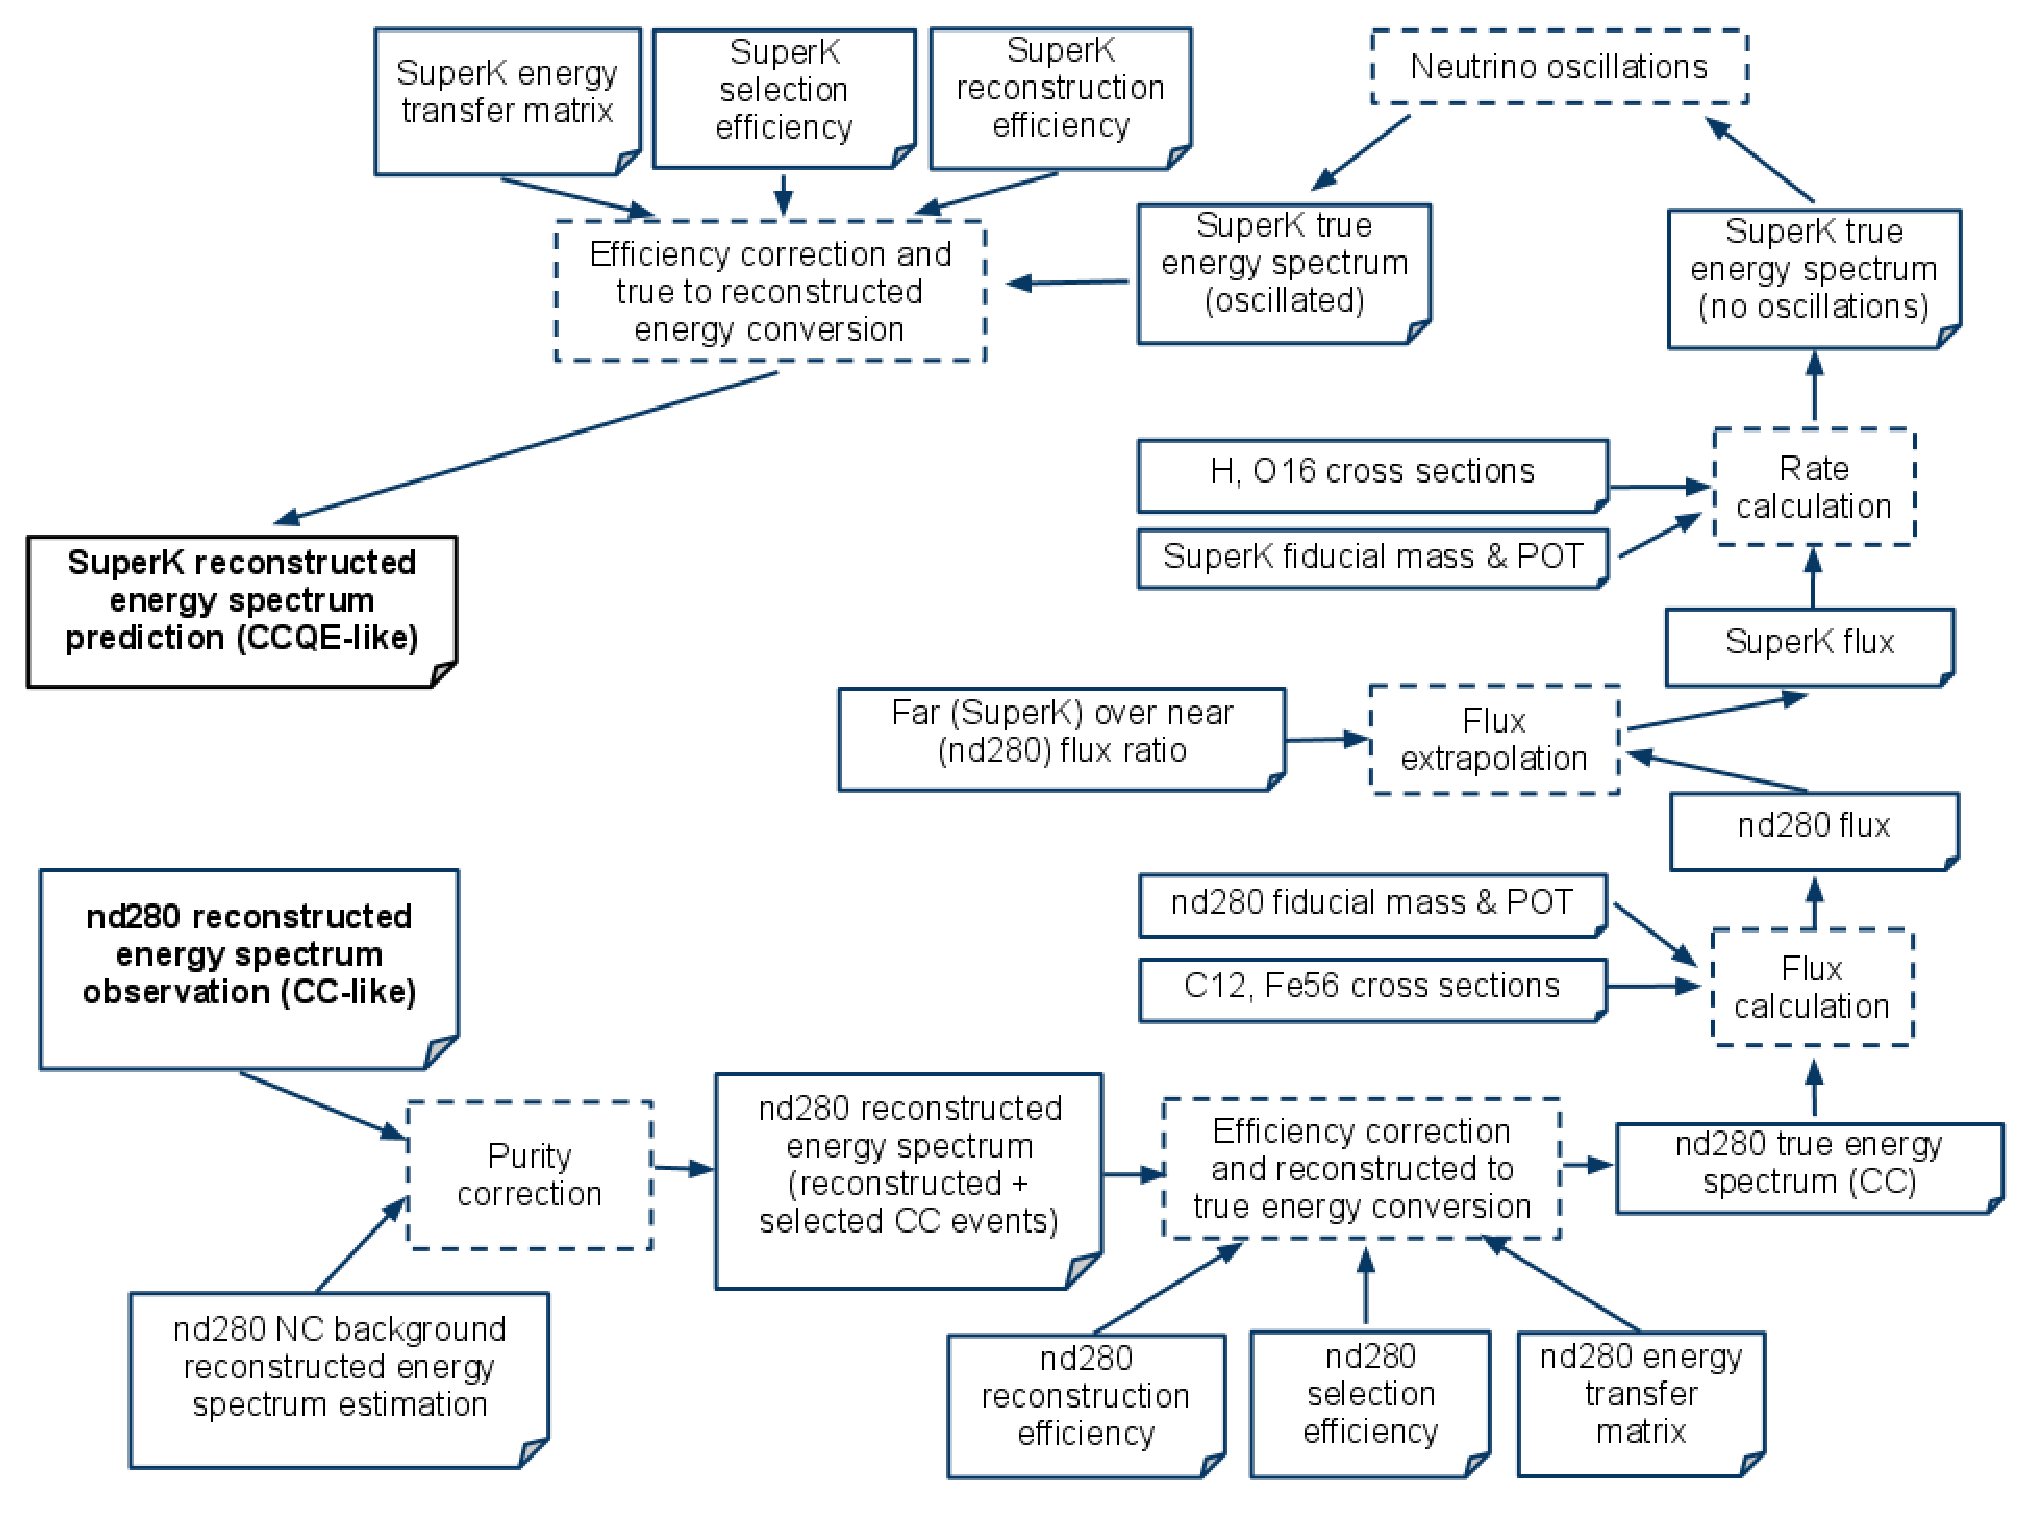
\includegraphics[width=38pc]{./images/analysis_steps.eps}
\caption{
  Outline of the procedure for predicting the SuperK reconstructed energy spectrum 
  of $\nu_{\mu}$ CCQE-like events
  from the $\nu_{\mu}$ CC inclusive reconstructed energy spectrum 
  measured in ND280.
}
\label{fig:AnalysisSteps}
\end{figure*}

The predicted reconstructed energy ($E_{r}$) spectrum ($\frac{dN_{SK}^{exp}}{dE_{r}}$) 
of selected 1 $\mu$-like ring events at SuperK,
is the sum of the corresponding spectra for all event types $m$\footnote{
 In this work, 
  $m$ = $\nu_{\mu}$ CCQE, $\nu_{\mu}$ CC1$\pi$, $\nu_{\mu}$ CC other, $\nu_{\mu}$($\nu_{\tau}$) NC, 
  $\bar{\nu_{\mu}}$ CCQE, $\bar{\nu_{\mu}}$ CC1$\pi$, $\bar{\nu_{\mu}}$ CC other $\bar{\nu_{\mu}}$($\bar{\nu_{\tau}}$) NC, 
  $\nu_{e}$ CCQE, $\nu_{e}$ CC1$\pi$, $\nu_{e}$ CC other and  $\nu_{e}$ NC.
} 
whose contribution is tracked separately.

\begin{equation}
\displaystyle
  \frac{dN_{SK}^{exp}(E_{r})}{dE_{r}} =
     \sum_{m} \frac{dN_{SK;m}^{exp}(E_{r})}{dE_{r}} 
\end{equation}

Let 
$\epsilon^{reco}_{SK;m}(E_{t})$
be the SuperK efficiency for reconstructing a neutrino event of type $m$ and true energy $E_{t}$, 
and 
$\epsilon^{sel}_{SK;m}(E_{r})$ be the SuperK efficiency for selecting an event of type $m$
and reconstructed energy $E_{r}$.
If $R_{SK;m}(E_{t},E_{r})$ is the SuperK energy transfer matrix\footnote{
The quantity $R_{SK;m}(E_{t},E_{r})$ is defined by
\begin{equation}
\displaystyle
   \frac{dN_{SK;m}}{dE_{r}}
 = \int { dE_{t} \frac{d^{2}N_{SK;m}}{dE_{r}dE_{t}} }
 = \int { dE_{t} \frac{dN_{SK;m}}{dE_{t}} R_{SK;m} }
\end{equation}
This implies that
\begin{equation}
\displaystyle
    R_{SK;m} 
 = \frac{d^{2}N_{SK;m}}{dE_{r}dE_{t}} / 
    \frac{dN_{SK;m}}{dE_{t}}
\end{equation}
This also defines the normalization properties all the $R_{SK;m}(E_{t},E_{r})$ matrix:
the elements for each $E_{r}$ row (or column, depending on how the matrix is represented) should add up to 1.
}
for events of type $m$, the expected reconstructed energy spectrum can be expressed in terms of the
total true neutrino energy spectrum
($\frac{dN_{SK;m}^{tot}(E_{t})}{dE_{t}}$):

\begin{equation}
\displaystyle
  \frac{dN_{SK}^{exp}(E_{r})}{dE_{r}} 
  = \sum_{m} \int dE_{t} 
    \frac{dN_{SK;m}^{tot}(E_{t})}{dE_{t}} 
    R_{SK;m}(E_{t},E_{r}) 
    \epsilon^{sel}_{SK;m}(E_{r}) 
    \epsilon^{reco}_{SK;m}(E_{t})
\end{equation}

The above expression can be rewritten to explicitly include
the survival probability $P_{m}^{surv}(E_{t})$ for neutrinos of energy $E_{t}$,
and the total non-oscillated true neutrino energy spectrum $\frac{dN_{SK;m}^{tot;unosc}}{dE_{t}}$:
\begin{equation}
\displaystyle
  \frac{dN_{SK}^{exp}(E_{r})}{dE_{r}} 
  = \sum_{m} \int dE_{t} 
    \frac{\displaystyle dN_{SK;m}^{tot;unosc}(E_{t})}
         {\displaystyle dE_{t}} 
    P_{m}^{surv}(E_{t}) 
    R_{SK;m}(E_{t},E_{r}) 
    \epsilon^{sel}_{SK;m}(E_{r}) 
    \epsilon^{reco}_{SK;m}(E_{t})
\end{equation}

The total non-oscillated true neutrino energy spectrum is related to
the estimated neutrino flux at SuperK
($\frac{d\Phi_{SK}(E_{t})}{dE_{t}}$) in the following way:
{
\arraycolsep=2pt
\begin{equation}
\displaystyle
\begin{array}{lcl}
  \frac{dN_{SK}^{exp}(E_{r})}{dE_{r}}  & = & 
    N_{SK}^{POT} M_{SK}^{fid} \frac{N_{A}}{A_{H20}}
    {\displaystyle \sum_{m} \int dE_{t}} \Bigg( 
    \frac{d\Phi_{SK}(E_{t})}{dE_{t}} \times \\ & &
    \sigma_{H20}^{tot}(E_{t}) 
    f_{m}(E_{t}) 
    P_{m}^{surv}(E_{t}) 
    R_{SK;m}(E_{t},E_{r}) 
    \epsilon^{sel}_{SK;m}(E_{r}) 
    \epsilon^{reco}_{SK;m}(E_{t}) \Bigg)
\end{array}
\label{eq:rate_sk}
\end{equation}
}
where 
$N_{SK}^{POT}$ is the proton-on-target exposure for the analyzed
SuperK data sample,
$M_{SK}^{fid}$ is the SuperK fiducial volume mass,
$\sigma_{H20}^{tot}(E_{t})$ is the total neutrino interaction cross section in water at energy $E_{t}$, 
$f_{m}(E_{t}$ is the fraction of events of type $m$,
$N_{A}$ is Avogadro's number and $A_{H20}$ is the water mass number.

The absolute neutrino flux $\frac{d\Phi_{SK}(E_{t})}{dE_{t}}$
in Eq. \ref{eq:rate_sk}, for which significant uncertainties exist,
can be constrained if it is expressed in terms of 
the observed reconstructed neutrino energy spectrum from an ND280 
inclusive charged-current sample.
From the definition of the far-over-near ratio

\begin{equation}
\displaystyle
  \frac{d\Phi_{SK}(E_{t})}{dE_{t}} = 
    R^{F/N}(E_{t}) \frac{d\Phi_{ND280}(E_{t})}{dE_{t}}
\end{equation}

where $\frac{d\Phi_{ND280}(E_{t})}{dE_{t}}$ is the neutrino flux at ND280.
This latter quantity can be related to the total CC true neutrino energy spectrum
$\frac{dN_{ND280;CC}^{tot}(E_{t})}{dE_{t}}$ as follows:

\begin{equation}
\displaystyle
  \frac{d\Phi_{SK}(E_{t})}{dE_{t}} = 
  \frac{R^{F/N}(E_{t}) A_{ND280}}{N_{ND280}^{POT} M_{ND280}^{fid} N_{A} \sigma^{CC}_{ND280}(E_{t})} 
  \frac{dN_{ND280;CC}^{tot}(E_{t})}{dE_{t}}
\end{equation}

where 
$N_{ND280}^{POT}$ is the proton-on-target exposure for the analyzed
ND280 data sample,
$M_{ND280}^{fid}$ is the fiducial mass for the ND280 `target' region, $\sigma^{CC}_{ND280}(E_{t})$ is the total 
charged-current cross section for the ND280 `target' region mixture at energy $E_{t}$
and $A_{ND280}$ is the mass number for the ND280 `target' mixture.

The total CC true neutrino energy spectrum can be expressed in terms
of the observed
reconstructed neutrino energy spectrum (which has the NC background subtracted):
{
\arraycolsep=2pt
\begin{equation}
\displaystyle
\begin{array}{lcl}
  \frac{d\Phi_{SK}(E_{t})}{dE_{t}} & = & 
  \frac{R^{F/N}(E_{t}) A_{ND280}}{N_{ND280}^{POT} M_{ND280}^{fid} \sigma^{CC}_{ND280}(E_{t})}
  {\displaystyle \int dE_{r\prime}} \Bigg( \\ & &
    \Big(
      \frac{dN_{ND280;CC-like}^{obs}(E_{r\prime})}{dE_{r\prime}} - 
      \frac{dN_{ND280;NC-bkg}^{exp}(E_{r\prime})}{dE_{r\prime}}
    \Big)  
    \frac{R^{T}_{ND280;CC}(E_{t},E_{r\prime})}
         {\epsilon^{reco}_{ND280;CC}(E_{t}) \epsilon^{sel}_{ND280;CC}(E_{r\prime})}
  \Bigg)
\end{array}
\label{eq:flux_sk}
\end{equation}
}
where
$\epsilon^{reco}_{ND280;CC}(E_{t})$ is the ND280 efficiency for reconstructing a charged-current neutrino event with true energy $E_{t}$,
$\epsilon^{sel}_{ND280;CC}(E_{r\prime})$ is the ND280 selection efficiency for a charged-current event reconstructed with energy $E_{r\prime}$, and
$R^{T}_{ND280;CC}(E_{t},E_{r\prime})$ is the transpose of the ND280 energy transfer matrix for charged-current events.

Combining Eq. \ref{eq:rate_sk} and \ref{eq:flux_sk} we obtain
{
\arraycolsep=2pt
\begin{equation}
\displaystyle
\begin{array}{lcl}
  \frac{dN_{SK}^{exp}(E_{r})}{dE_{r}} & = & 
  \frac{N_{SK}^{POT} M_{SK}^{fid} A_{ND280}}{N_{ND280}^{POT} M_{ND280}^{fid} A_{H20}} 
  {\displaystyle \sum_{m} \int dE_{t} \int dE_{r\prime}} \Bigg( 
  R^{F/N}(E_{t})
  \frac{\sigma_{H20}^{tot}(E_{t}) f_{m}(E_{t})}{\sigma^{CC}_{ND280}(E_{t})}
  P_{m}^{surv}(E_{t}) \times \\ & &
  \Big(\frac{dN_{ND280;CC-like}^{obs}(E_{r\prime})}{dE_{r\prime}} - 
       \frac{dN_{ND280;NC-bkg}^{exp}(E_{r\prime})}{dE_{r\prime}}\Big)  \times \\ & &
    R_{SK;m}(E_{t},E_{r}) R^{T}_{ND280;CC}(E_{t},E_{r\prime}) 
    \frac{\epsilon^{sel}_{SK;m}(E_{r}) \epsilon^{reco}_{SK;m}(E_{t})}
         {\epsilon^{reco}_{ND280;CC}(E_{t}) \epsilon^{sel}_{ND280;CC}(E_{r\prime})} 
    \Bigg)
\end{array}
\label{eq:far_prediction}
\end{equation}%
}

%
% Implementation / analysis specifics
%

\subsection {3.23$\times10^{19}$-POT analysis specifics and discussion of ND280 input}
\label{sec:superkprediction_analysis_specifics}

In the present analysis, there is no spectral information in the inclusive CC ND280 measurement.
In this case, Eq. \ref{eq:far_prediction} simplifies to
\begin{equation}
\displaystyle
\begin{array}{lcl}
  \frac{dN_{SK}^{exp}(E_{r})}{dE_{r}}  & = & 
    N_{SK}^{POT} M_{SK}^{fid} \frac{N_{A}}{A_{H20}}
    C_{ND280}
    {\displaystyle \sum_{m} \int dE_{t}} \Bigg( 
    \\ & &
    \frac{d\Phi_{SK}(E_{t})}{dE_{t}} 
    \sigma_{H20}^{tot}(E_{t}) 
    f_{m}(E_{t}) 
    P_{m}^{surv}(E_{t}) 
    R_{SK;m}(E_{t},E_{r}) 
    \epsilon^{sel}_{SK;m}(E_{r}) 
    \epsilon^{reco}_{SK;m}(E_{t}) \Bigg)
\end{array}
\label{eq:far_prediction_no_nd280_spectrum}
\end{equation}
where $C_{ND280}$ is the ND280 data-driven correction factor on the flux times cross section product.
We note that the far over near ratio $R^{F/N}(E_{t})$, discussed previously, does not appear in the above formula.
This follows from the fact that the ND280 measurement has no energy dependence.

In Eq. \ref{eq:far_prediction_no_nd280_spectrum}, $C_{ND280}$ is given by
\begin{equation}
\displaystyle
  C_{ND280} = 
    \frac{N^{obs}_{ND280;CC-like}}
         {N^{exp}_{ND280;CC}+N^{exp}_{ND280;NC-bkg}}
\label{eq:nd280correction}
\end{equation}
where
$N^{obs}_{ND280;CC-like}$ is the observed number of CC-like events,
$N^{exp}_{ND280;NC-bkg}$ is the expected NC contamination of the observation, and
$N^{exp}_{ND280;CC}$ is the expected number of CC events.

In the present analysis 
$C_{ND280}$ is 1.1549 for GENIE and 1.06127 for NEUT\cite{ND280AnalysisInputs,ND280ClaudioThesis}.
The difference in the required correction factor for GENIE and NEUT reflects 
generator-level tuning choices; mainly, it reflects the dramatic difference in the choice of the input CCQE axial mass.
The authors of GENIE use a value of $M_{A}$ = 0.99 GeV/$c^{2}$ which is better-motivated theoretically.
One the other hand, the authors of NEUT use a higher value ($M_{A}$ = 1.2 GeV/$c^{2}$) 
motivated by K2K and MiniBooNE measurements of an increased event rate (in $C^{12}$, $O^{16}$ targets)
compared with expectations informed by previous measurements in deuterium targets (although the observed excess
is only about 1$\sigma$). It is plausible, although not satisfying, that $M_{A}$ should have a larger
values for nuclear targets. However, it is also likely that the discrepancy is caused, amongst other things, 
by underestimating the K2K and MiniBooNE neutrino flux,
or by the existence of unmodelled CCQE-like contributions (2p2h).
So, increasing $M_{A}$ may or may not be appropriate.
The issue is far from being resolved and reflects a genuine physics uncertainty: 
the absolute neutrino cross section at around 1 GeV is known only to about 20-30\%.

In any case, this (or any) T2K oscillation analysis is credible only if it is 
shown explicitly that it does not depend on semi-arbitrary generator choices,
and that measurements from the near detector suite effectively constrain uncertainties 
in the product of flux and cross-section. It also needs to be shown that any difference in
the oscillation results is well-understood in terms of the quoted cross-section systematics.
This is the main motivation behind pursuing this analysis using both GENIE and NEUT.


\subsection {Implementation details}

So far, the SuperK spectrum prediction method has been presented in a formal manner.
In practice, the procedure for calculating the spectrum can be simplified.
By using appropriate Monte Carlo `templates', representing the simulated number of
events in N-dimensional bins of kinematical quantities,
one can avoid performing integrations such as the one appearing 
in Eq. \ref{eq:rate_sk}\footnote
{
  On the SuperK side of the calculation, 
  avoiding integrations such as the one in Eq. \ref{eq:rate_sk} using MC templates
  is just a matter of convenience and computational efficiency.
  However, on the ND280 side, avoiding such integrations and, instead, using MC templates 
  is a necessity.
  Indeed, for ND280, event rate calculations folding in the flux and neutrino cross section to
  should be generalized to take into account the effects arising from the convolution of a 
  non-uniform flux with non-uniform detector mass distribution. In this case, the event rate
  can be written as
  \begin{equation}
    \displaystyle
       N^{exp} = N^{POT} N_{A} 
            \int d^{3}x \int d^{3}p 
            \frac{d^{6}\Phi({\bf x},{\bf p})}{d^{3}xd^{3}p} 
            \epsilon(E) 
            \sum_{a} \frac{\sigma_{a}(E)}{A_{a}} \int dl\rho_{a}
       \label{eq:event_rate_complex}
  \end{equation}
  where 
  the vector ${\bf x}$ is the flux neutrino point of origin and
  the vector ${\bf p}$ is the flux neutrino momentum.
  In the above equation, the sum over $a$ is the sum over nuclear targets in the detectors.
  The mass number of each nuclear target is $A_{a}$ and the total interaction cross section is $\sigma_{a}(E)$.
  The final integral in Eq. \ref{eq:event_rate_complex} calculates the density-weighted path length
  for nuclear target $a$ with density $\rho_{a}$ along the given flux netrino trajectory.
  This complicated integration is already performed by GENIE and NEUT using Monte Carlo techniques
  and the result is built into the generated templates.
  It is practically impossible and unnecessary to reproduce this time-consuming Monte Carlo
  integration in the context of the oscillation analysis.
}

In this analysis, 
oscillation parameters are determined by fitting the reconstructed energy ($E_{r}$) spectrum
of 1-ring $\mu$-like events observed at SuperK, 
oscillation weights are functions of the true energy ($E_{t}$),
and all considered systematics affecting the SuperK spectrum prediction
either have no kinematical dependence or depend 
on only one of true or reconstructed energy.
Therefore, in the context of this analysis, it is sufficient to use 2-dimensional
templates representing the number of SuperK events, as estimated by MC,
as functions of $E_{r}$ and $E_{t}$.
Let $N_{SK;m;r;t}^{MC}$ be such a template for events of mode $m$ in the 1 $\mu$-like ring sample,
where indices $r$ and $t$ denote, respectively, reconstructed and true energy bin numbers.
The construction of these templates is discussed in detail in Sec. \ref{sk_templates}.
The predicted number $N_{SK;r}^{exp}$ 
of SuperK events in the $r^{th}$ reconstructed energy bin
can be written in terms of the $N_{SK;m;r;t}^{MC}$ templates as
\begin{equation}
\displaystyle
  N_{SK;r}^{exp} = 
    C_{ND280}
    \sum_{m} \sum_{t} 
    	P_{m;t}^{surv}
	N_{SK;m;r;t}^{MC}
\label{eq:far_prediction_no_nd280_spectrum_with_sk_templates}
\end{equation}
where $C_{ND280}$ is the ND280 correction factor defined in Eq. \ref{eq:nd280correction}
and $P_{m;t}^{surv}$ is oscillation survival probability applied in the $t^{th}$ true energy
bin of the SuperK MC template which corresponds to mode $m$.
Application of term $P_{m;t}^{surv}$ is discussed in Sec. \ref{applying_oscillations}.

Only the value of $C_{ND280}$ is needed for the prediction of the nominal SuperK spectrum.
However, for systematic studies, one needs to be able to calculate how the value of $C_{ND280}$ 
is modified as a result of systematic parameter variations.
Therefore it is necessary to express $C_{ND280}$ in terms of appropriate ND280 MC templates.
In this analysis, all considered systematics affecting $C_{ND280}$
either have no kinematical dependence or depend on true energy only.
Therefore, in the context of this analysis, it is sufficient to use 1-dimensional
templates representing the number of ND280 events, as estimated by MC,
as functions of $E_{t}$.
Let $N_{ND280;m\prime;t}^{MC}$ be such a template for events of mode $m\prime$ in the
ND280 CC inclusive sample, where index $t$ denotes true energy bin number.
The construction of these templates is discussed in Sec. \ref{nd280_templates}.
Using the ND280 MC templates, $C_{ND280}$ can be written as
\begin{equation}
\displaystyle
  C_{ND280} = N^{obs}_{ND280;CC-like} / \sum_{m\prime} N^{MC}_{ND280;m\prime}
\label{eq:nd280correction_with_templates}
\end{equation}

Using Eq. \ref{eq:nd280correction_with_templates}, 
Eq. \ref{eq:far_prediction_no_nd280_spectrum_with_sk_templates} can be written as
\begin{equation}
\displaystyle
  N_{SK;r}^{exp} = 
    (N^{obs}_{ND280;CC-like} /
     \sum_{m\prime} N^{MC}_{ND280;m\prime})
    \cdot 
    \sum_{m} \sum_{t} 
    	P_{m;t}^{surv}
	N_{SK;m;r;t}^{MC}
\label{eq:far_prediction_no_nd280_spectrum_final}
\end{equation}
This is the actual formula used in this analysis for predicting the 
SuperK reconstructed energy spectrum.

\subsection{Construction of SuperK MC templates}
\label{sk_templates}

The $N_{SK;m;r;t}^{MC}$ templates are shown in Fig. \ref{fig:genie_etrue_ereco_templates} (GENIE) 
and Fig. \ref{fig:neut_etrue_ereco_templates} (NEUT). Separate templates are used for
$\nu_{\mu}$ CCQE\footnote{
  A commonly asked question is why the $\nu_{\mu}$-CCQE template is not just a `line' along
  the diagonal. Conservation of energy and momentum is the anwer to this question.
  Recall that the $\nu_{\mu}$-CCQE template is generated from a sample of $\nu_{\mu}$ interactions
  in water and that, in oxygen, the Fermi level $k_{F}$ is 225 MeV.
  On the other hand, recall that the hit bound-nucleon momentum is `esoteric' 
  and that the reconstructed neutrino energy formula naturally assumes that the hit nucleon was at rest.
}, 
$\nu_{\mu}$ CC1$\pi$, 
$\nu_{\mu}$ CC other, 
$\nu_{\mu}$($\nu_{\tau}$) NC, 
$\bar{\nu_{\mu}}$ CCQE, 
$\bar{\nu_{\mu}}$ CC1$\pi$, 
$\bar{\nu_{\mu}}$ CC other, 
$\bar{\nu_{\mu}}$($\bar{\nu_{\tau}}$) NC, 
$\nu_{e}$ CCQE, 
$\nu_{e}$ CC1$\pi$,
$\nu_{e}$ CC other and 
$\nu_{e}$ NC.
The events contributing to the construction of these 2-D templates are the ones that
pass the `1-ring $\mu$-like (tight)' cuts. The templates span the 0-10 GeV range in
both $E_{r}$ and $E_{t}$ variables using 50 MeV bins.

The templates were generated using the 2010a GENIE and NEUT SuperK samples and
then they were reweighted to the 2010d(v2) flux \cite{BeamWeights10dv2}.
Details of the 2010a GENIE and NEUT SuperK samples and of the applied selection cuts are given below.

\subsubsection*{SuperK MC samples}

\begin{itemize}
\item
GENIE SuperK sample:\\
 The 2010a GENIE SuperK Monte Carlo sample was generated at the Rutherford Appleton Laboratory
 PPD Tier2 cluster using GENIE v2.6.0 and the 2010a JNUBEAM flux \cite{BeamFlux10a}.
 The GENIE decay flags for $D^{+}$, $D^{-}$, $D^{0}$, $\bar{D^{0}}$, $D_{s}^{+}$, $D_{s}^{-}$,
 $\Lambda_{c}^{+}$, $\Sigma_{c}^{0}$, $\Sigma_{c}^{+}$ and $\Sigma_{c}^{++}$ 
 were set to `true' (non-default GENIE settings) as the SuperK detector simulation would not
 decay charmed hadrons. Default GENIE v2.6.0 values were used for all other physics options.

 The GENIE vector files were proccessed by P. de Perio at the SciNet cluster in Toronto.
 The SK software used is the same as that used for the official 10a NEUT production
 (SKDETSIM-v11p79\_for\_atmnu\_apr10, ATMPD-10a, SKOFL-10a, ROOT-v5.26) \cite{PatrickPrivComm}.
 The `T2K PMT flasher reduction' cut was not included when filling the output DSTs.
 According to experts `this is a small effect ( $<$ 1\% )' \cite{SuperKFC}.

 Using the GENIE v2.6.0 cross section calculations for water and the 2010a JNUBEAM flux,
 we calculate
 1325.4200 $\nu_{\mu}$       events / 22.5 kt fiducial mass / $10^{21}$ POT,
   65.1023 $\bar{\nu_{\mu}}$ events / 22.5 kt fiducial mass / $10^{21}$ POT and
   25.9600 beam $\nu_{e}$    events / 22.5 kt fiducial mass / $10^{21}$ POT.
 After applying fiducial volume cuts to the generated samples, we find that
   604403 $\nu_{\mu}$,
   303747 $\bar{\nu_{\mu}}$ and
   621525 beam $\nu_{e}$  
 events have survived.
 From the above, we calculate the following absolute normalizations 
 for the 2010a samples:
   4.560000$\times10^{23}$ POT for the $\nu_{\mu}$ sample,
   4.665680$\times10^{24}$ POT for the $\bar{\nu_{\mu}}$ sample and
   2.394164$\times10^{25}$ POT for the beam $\nu_{e}$ sample.
 Therefore, the MC scaling factors to the data beam exposure ($3.23\times10^{19}$ POT) are
   7.08333$\times10^{-5}$ ($\nu_{\mu})$,
   6.92289$\times10^{-6}$ ($\bar{\nu_{\mu}}$),
   1.34911$\times10^{-6}$ (beam $\nu_{e}$). 
   
\item
NEUT SuperK sample:\\
 The 2010a NEUT SuperK Monte Carlo sample was generated and processed at the Kamioka cluster.
 NEUT v5.0.7 and the 2010a JNUBEAM flux were used.
 The corresponding SuperK DSTs were kindly provided by P. de Perio.
 The MC scaling factors to the data POT exposure are the ones provided by Y.Hayato and J.Kameda \cite{KamedaPrivComm}:
   7.35361$\times10^{-5}$ ($\nu_{\mu})$,
   7.17816$\times10^{-6}$ ($\bar{\nu_{\mu}}$),
   1.48428$\times10^{-6}$ (beam $\nu_{e}$). 

\end{itemize}

\subsubsection*{SuperK selection cuts}

The standard SuperK cuts for obtaining
a) `fully contained fiducial volume (FCFV)',
b) `1 $\mu$-like ring',
c) `1 $\mu$-like ring (tight)' and
d) `$>$ 1 $\mu$-like ring'
samples are shown in Tab. \ref{tab:NuMuEventSelections}.
In this analysis, the 1 $\mu$-like ring (tight) event selection is used.

\begin{table}
\centering
\begin{tabular}{| c | c | c | c |}
\hline
Fully contained & 1 $\mu$-like ring & 1 $\mu$-like ring & $>$ 1 $\mu$-like ring  \\
fiducial volume &  & (tight) & \\
\hline
\hline
Number of PMT hits  & Number of PMT hits  &  Number of PMT hits  &  Number of PMT hits \\
in highest charge   & in highest charge   &  in highest charge   &  in highest charge  \\
Outer Detector      & Outer Detector      & Outer Detector       & Outer Detector      \\
cluster $<$= 15     & cluster $<$= 15     & cluster $<$= 15      & cluster $<$= 15     \\
\hline
Vertex $>$ 2m from  & Vertex $>$ 2m from  & Vertex $>$ 2m from   & Vertex $>$ 2m from  \\
Inner Detector wall & Inner Detector wall & Inner Detector wall  & Inner Detector wall \\
\hline
E$_{visible}$ $>$ 30 MeV & E$_{visible}$ $>$ 30 MeV & E$_{visible}$ $>$ 30 MeV & E$_{visible}$ $>$ 30 MeV \\
\hline
  & Exactly 1 ring & Exactly 1 ring & $>$ 1 ring \\
\hline
 & ip[0] = 3 & ip[0] = 3 & Ring with largest \\
 & ($\mu$-like ring) & ($\mu$-like ring) & amome is $\mu$-like \\
\hline
 &  & amomm[0] $>$ & \\
 &  & 200 MeV & \\
\hline
 &  & $<$= 1 decay e$^{-}$  & \\
\hline
\end{tabular}
\caption{
 Standard SuperK $\nu_{\mu}$ event selection cuts. In this analysis, the 1-ring $\mu$-like (tight) event selection is used.
 Potential benefits from including the multi-ring $\mu$-like events will be explored in future revision
 of this work.
}
\label{tab:NuMuEventSelections}
\end{table}

\begin{figure*}[htb]
\center
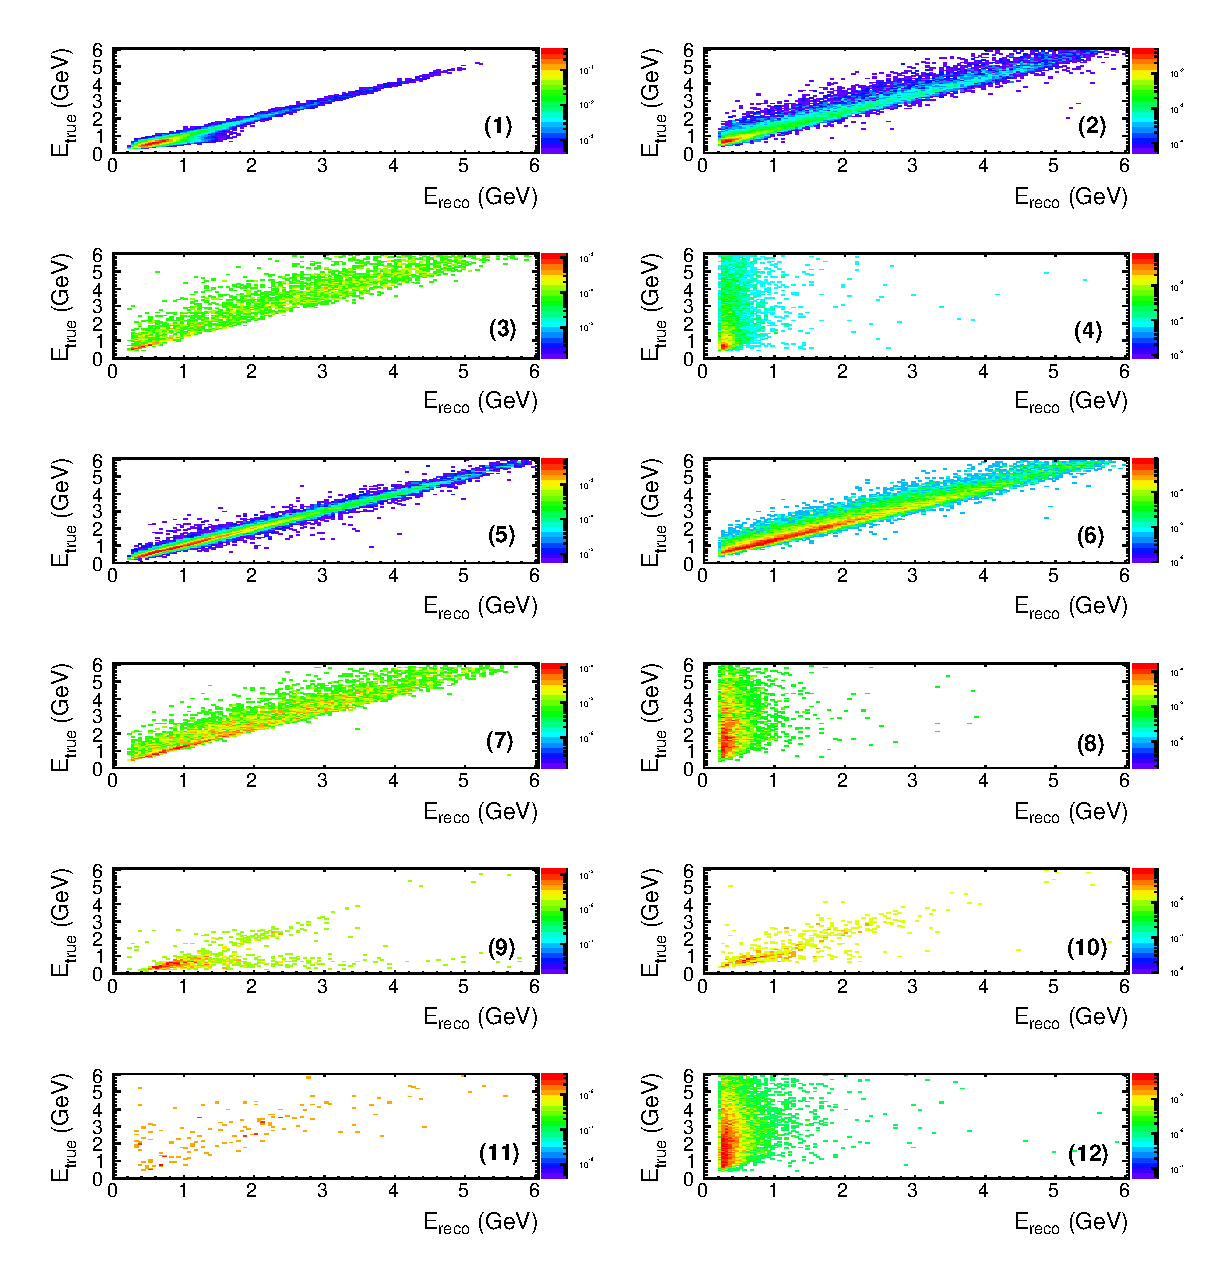
\includegraphics[width=38pc]{./images/templates/genie_etrue_ereco_templates.eps}
\caption{
  GENIE ($E_{t}$, $E_{r}$) 1-ring $\mu$-like MC templates. 
  The templates are shown for
  $\nu_{\mu}$ CCQE (1), 
  $\nu_{\mu}$ CC1$\pi$ (2), 
  $\nu_{\mu}$ CC other (3), 
  $\nu_{\mu}$($\nu_{\tau}$) NC (4), 
  $\bar{\nu_{\mu}}$ CCQE (5), 
  $\bar{\nu_{\mu}}$ CC1$\pi$ (6), 
  $\bar{\nu_{\mu}}$ CC other (7), 
  $\bar{\nu_{\mu}}$($\bar{\nu_{\tau}}$) NC (8), 
  $\nu_{e}$ CCQE (9),
  $\nu_{e}$ CC1$\pi$ (10),
  $\nu_{e}$ CC other (11) and
  $\nu_{e}$ NC (12).
  The templates are zoomed-in for illustration purposes. 
  The range 0-10 GeV is used in the analysis.
}
\label{fig:genie_etrue_ereco_templates}
\end{figure*}

\begin{figure*}[htb]
\center
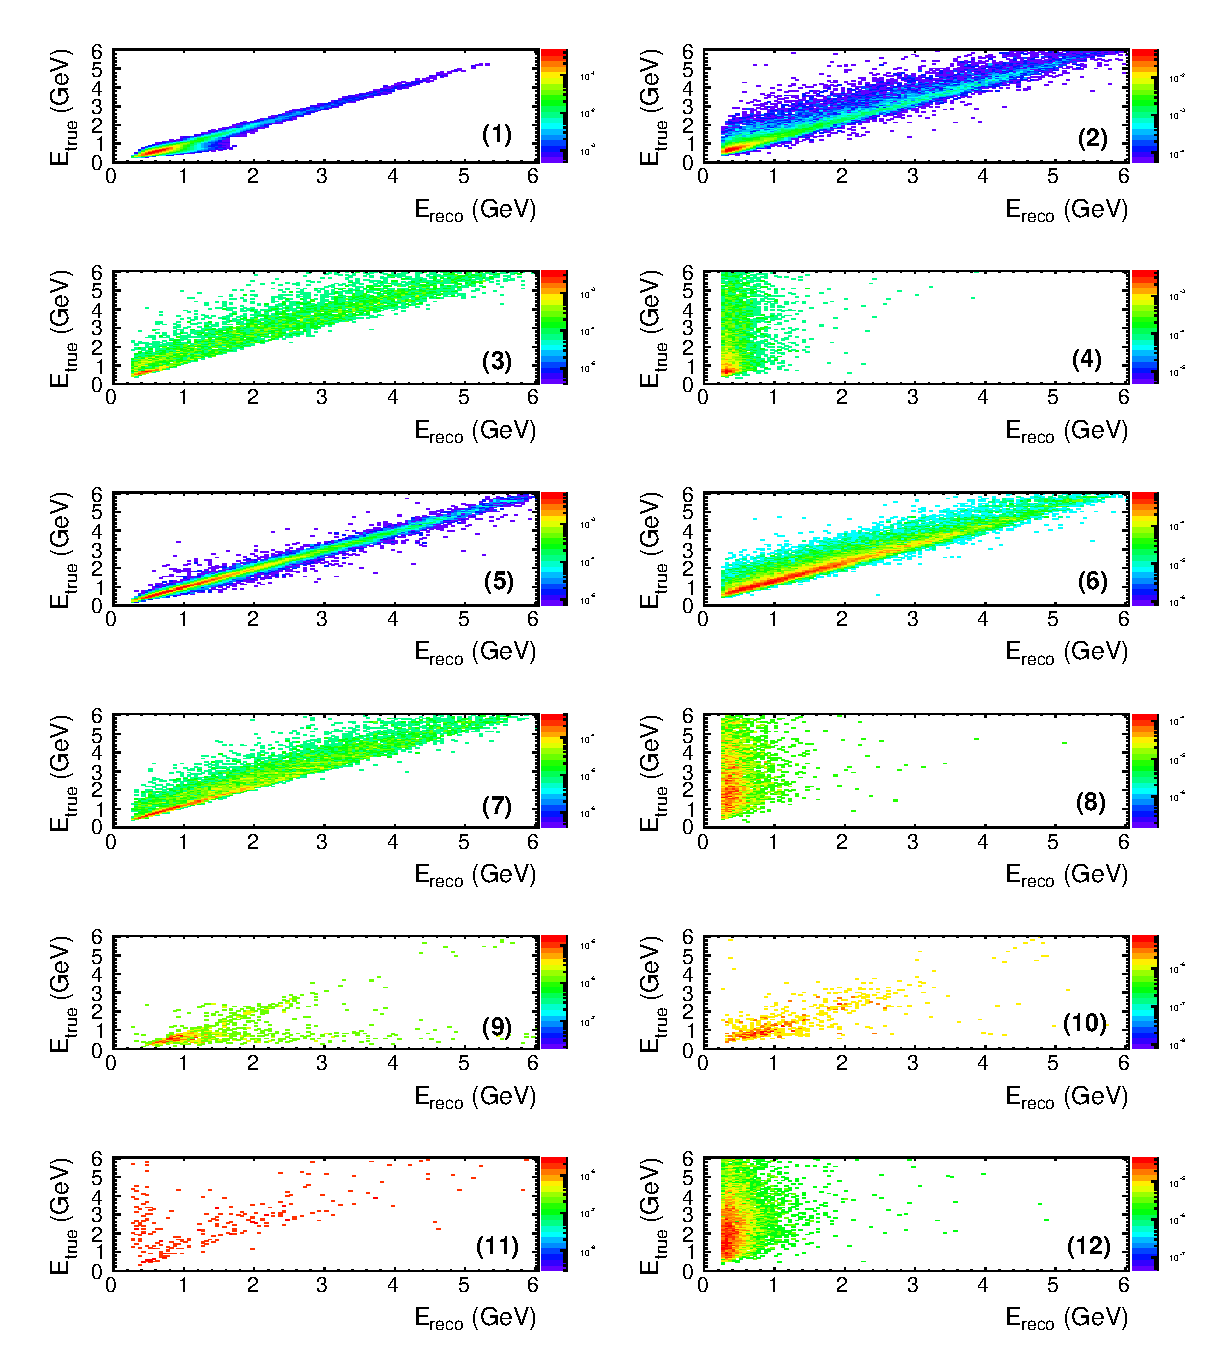
\includegraphics[width=38pc]{./images/templates/neut_etrue_ereco_templates.eps}
\caption{
  NEUT ($E_{t}$, $E_{r}$) 1-ring $\mu$-like MC templates. 
  The order of templates is the same as in Fig.\ref{fig:genie_etrue_ereco_templates}.
}
\label{fig:neut_etrue_ereco_templates}
\end{figure*}


\subsection{ND280 MC templates}
\label{nd280_templates}

The ND280 MC templates were provided directly by the ND280 group \cite{ND280AnalysisInputs}.
In total 21 histograms were provided representing the number of events as a function
of true energy for
1)  $\nu_{\mu}$ CC QE,	
2)  $\nu_{\mu}$ CC resonance,
3)  $\nu_{\mu}$ CC coherent,
4)  $\nu_{\mu}$ CC other,
5)  $\nu_{\mu}$ NC resonance,
6)  $\nu_{\mu}$ NC coherent,
7)  $\nu_{\mu}$ NC other,
8)  $\bar{\nu_{\mu}}$ CC QE,
9)  $\bar{\nu_{\mu}}$ CC resonance,
10) $\bar{\nu_{\mu}}$ CC coherent,
11) $\bar{\nu_{\mu}}$ CC other,
12) $\bar{\nu_{\mu}}$ NC resonance,
13) $\bar{\nu_{\mu}}$ NC coherent,
14) $\bar{\nu_{\mu}}$ NC other,
15) $\nu_{e}$ CC QE,
16) $\nu_{e}$ CC resonance,
17) $\nu_{e}$ CC coherent,
18) $\nu_{e}$ CC other,
19) $\nu_{e}$ NC resonance,
20) $\nu_{e}$ NC coherent and
21) $\nu_{e}$ NC other.
These templates were generated by applying the Saclay CC inclusive selection cuts
to the ND280 MCP1 GENIE and NEUT samples. The GENIE and NEUT versions used in the
ND280 MCP1 production are the same as those used at the SuperK 2010a production.
They were reweighted to the 2010d(v2) flux \cite{BeamWeights10dv2}.
More details are given in \cite{ND280AnalysisInputs}.

\subsection{Applying neutrino oscillations}
\label{applying_oscillations}

Oscillations are applied to the 
$\nu_{\mu}$-CCQE, $\nu_{\mu}$-CC1$\pi$, $\nu_{\mu}$-CCother, 
$\bar{\nu_{\mu}}$-CCQE, $\bar{\nu_{\mu}}$-CC1$\pi$ and $\bar{\nu_{\mu}}$-CCother
MC templates (as function of $E_{t}$).
Oscillations are not applied to the $\nu_{\mu}$-NC and $\bar{\nu_{\mu}}$-NC MC templates
since they serve as proxies for the $\nu_{\mu}(+\nu_{\tau})$-NC and $\bar{\nu_{\mu}}(+\bar{\nu_{\tau}})$-NC MC templates
which are unchanged under 
$\nu_{\mu} \rightarrow \nu_{\tau}$ and 
$\bar{\nu_{\mu}} \rightarrow \bar{\nu_{\tau}}$ oscillations.
We neglect contributions from $\nu_{\tau}$-CC and $\bar{\nu_{\tau}}$-CC as their
energy threshold is around 3.5 GeV and their effect is negligible.
The effect of sub-dominant (and unknown) $\nu_{e}$ oscillation is also neglected.
The following oscillation survival probability is applied:
\begin{equation}
\displaystyle
  P_{surv} = 1 - sin^{2}{2\theta_{23}} \cdot 
                 sin^{2}\Big(
                  1.267 \cdot \frac{\Delta m^{2}_{23} (eV^{2}/c^{4}) \cdot 295.335 (km)}{E_{t} (GeV)}
                 \Big)
\label{eq:osc_formula}
\end{equation}
The same $sin^{2}{2\theta_{23}}$ and $\Delta m^{2}_{23}$ parameters 
are used for both $\nu_{\mu}$ and $\bar{\nu_{\mu}}$ oscillations.


%
% Event numbers
%

\clearpage

\subsection{Nominal GENIE and NEUT expectations under various oscillation hypotheses}

In this section we present plots and tables comparing the GENIE and NEUT SuperK predictions
(after extrapolation) under various oscillation hypotheses.
Figs. \ref{fig:genie_mode_contrib_noosc} and \ref{fig:neut_mode_contrib_noosc} show,
respectively, the GENIE and NEUT
predicted (after extrapolation) non-oscillated reconstructed-energy spectrum of 1-ring $\mu$-like events 
passing the tight cuts (see Tab. \ref{tab:NuMuEventSelections}). 
The contributions from various true neutrino reaction modes are also shown. 
The corresponding oscillated predictions 
($sin^{2}2\theta_{23}$=1.0 and $\Delta m^{2}_{23}$=2.4$\times10^{-3}$ $eV^{2}/c^{4}$)
are shown in 
Fig. \ref{fig:genie_mode_contrib_2p4Em3_1p0} for GENIE and 
Fig. \ref{fig:neut_mode_contrib_2p4Em3_1p0} for NEUT.
In Tab. \ref{tab:genie_neut_mode_contrib} we summarize 
Figs. \ref{fig:genie_mode_contrib_noosc} - \ref{fig:neut_mode_contrib_2p4Em3_1p0}.

In Fig. \ref{fig:genie_sk_spectrum_twk_sinsq2theta} we show the GENIE predicted 1-ring $\mu$-like event
reconstructed energy spectrum (after extrapolation) for a fixed $\Delta m^{2}_{23}$ and various $sin^{2}2\theta_{23}$ values.
The corresponding plot for NEUT is shown in Fig. \ref{fig:neut_sk_spectrum_twk_sinsq2theta}.
Tab. \ref{tab:genie_neut_nsk_twk_sinsq2theta} 
summarizes Figs. \ref{fig:genie_sk_spectrum_twk_sinsq2theta} and \ref{fig:neut_sk_spectrum_twk_sinsq2theta}.
In Fig. \ref{fig:genie_sk_spectrum_twk_dmsq} we show the GENIE predicted 1-ring $\mu$-like event
reconstructed energy spectrum (after extrapolation) for a fixed $sin^{2}2\theta_{23}$ and various $\Delta m^{2}_{23}$ values.
The corresponding plot for NEUT is shown in Fig. \ref{fig:neut_sk_spectrum_twk_dmsq}.
Tab. \ref{tab:genie_neut_nsk_twk_dmsq}
summarizes Figs. \ref{fig:genie_sk_spectrum_twk_dmsq} and \ref{fig:neut_sk_spectrum_twk_dmsq}.

In Fig. \ref{fig:genie_nsk_osc_param_grid} we show the GENIE predicted integrated number 
of 1-ring $\mu$-like events (after extrapolation) for a grid of $sin^{2}2\theta_{23}$ and $\Delta m^{2}_{23}$ values.
The corresponding plot for NEUT is shown in Fig. \ref{fig:neut_nsk_osc_param_grid}.
Finally, in Fig. \ref{fig:genie_neut_nsk_difference_osc_param_grid} we show
(for the same grid of $sin^{2}2\theta_{23}$ and $\Delta m^{2}_{23}$ values)
the percentage difference of the NEUT and GENIE predictions of integrated number 
of 1-ring $\mu$-like events (after extrapolation).


\begin{figure}[ht]
\begin{minipage}[t]{0.48\linewidth}
\centering
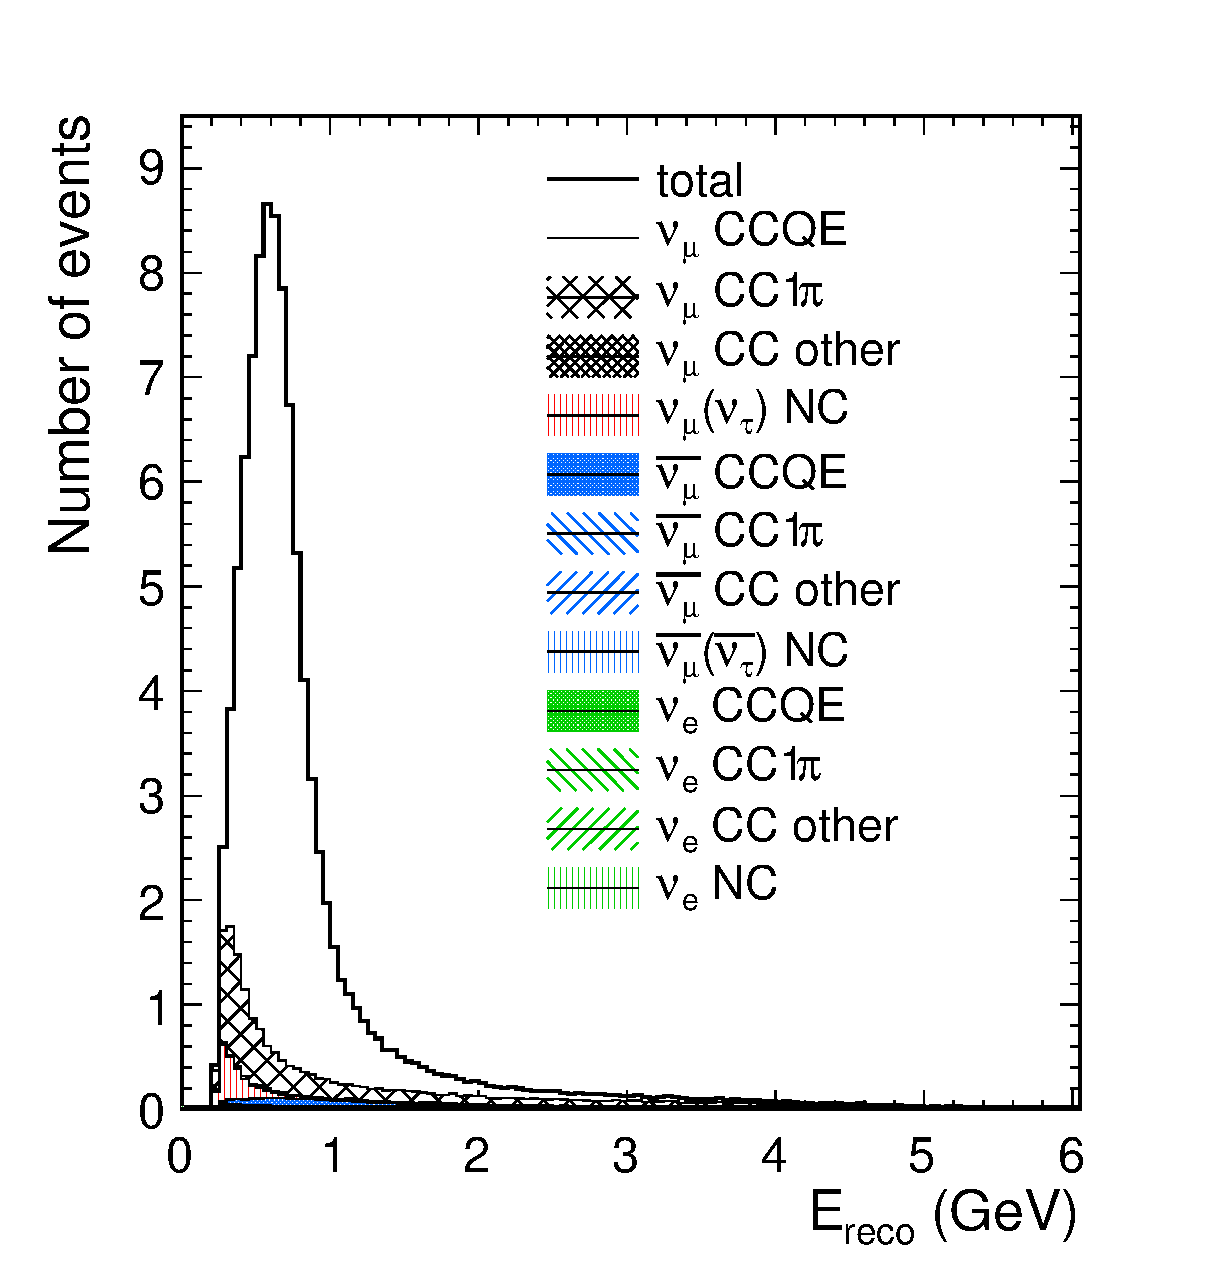
\includegraphics[width=19pc,height=19pc]{./images/predicted_spectrum/nominal/genie_contrib_noosc.eps}
\caption{
  Predicted non-oscillated reconstructed-energy spectrum of 1-ring $\mu$-like events (after extrapolation)
  and contributions from various true neutrino reaction modes (GENIE).
}
\label{fig:genie_mode_contrib_noosc}
\end{minipage}
\hspace{0.04\linewidth}
\begin{minipage}[t]{0.48\linewidth}
\centering
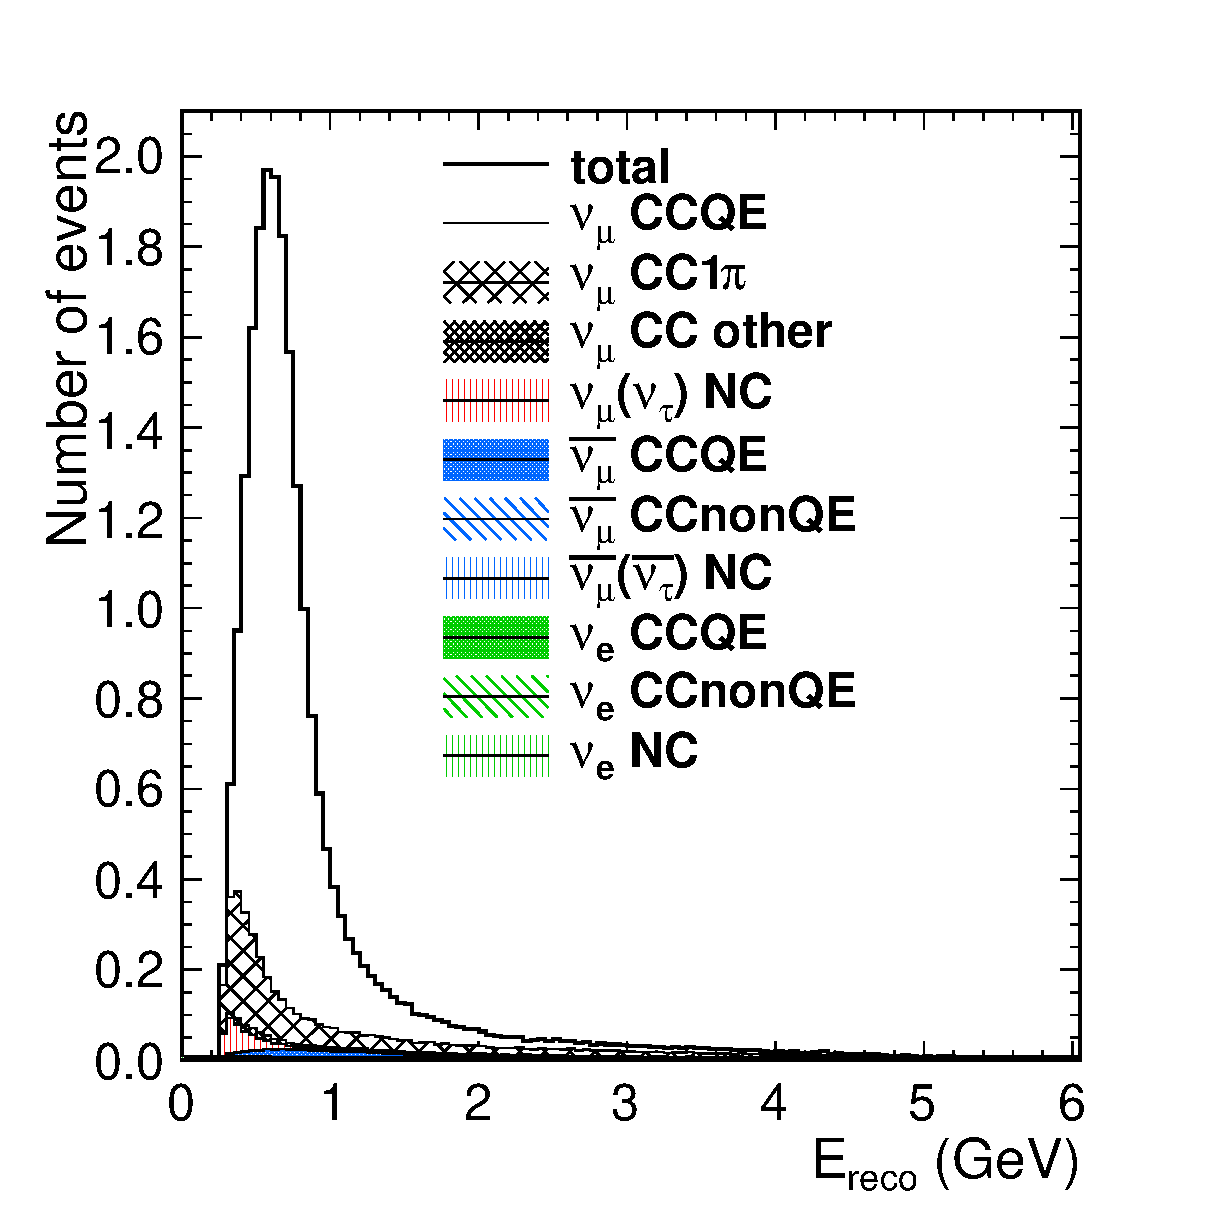
\includegraphics[width=19.5pc,height=19pc]{images/predicted_spectrum/nominal/neut_contrib_noosc.eps}
\caption{
  Predicted non-oscillated reconstructed-energy spectrum of 1-ring $\mu$-like events (after extrapolation)
  and contributions from various true neutrino reaction modes (NEUT).
}
\label{fig:neut_mode_contrib_noosc}
\end{minipage}
\end{figure}


\begin{figure}[ht]
\begin{minipage}[t]{0.48\linewidth}
\centering
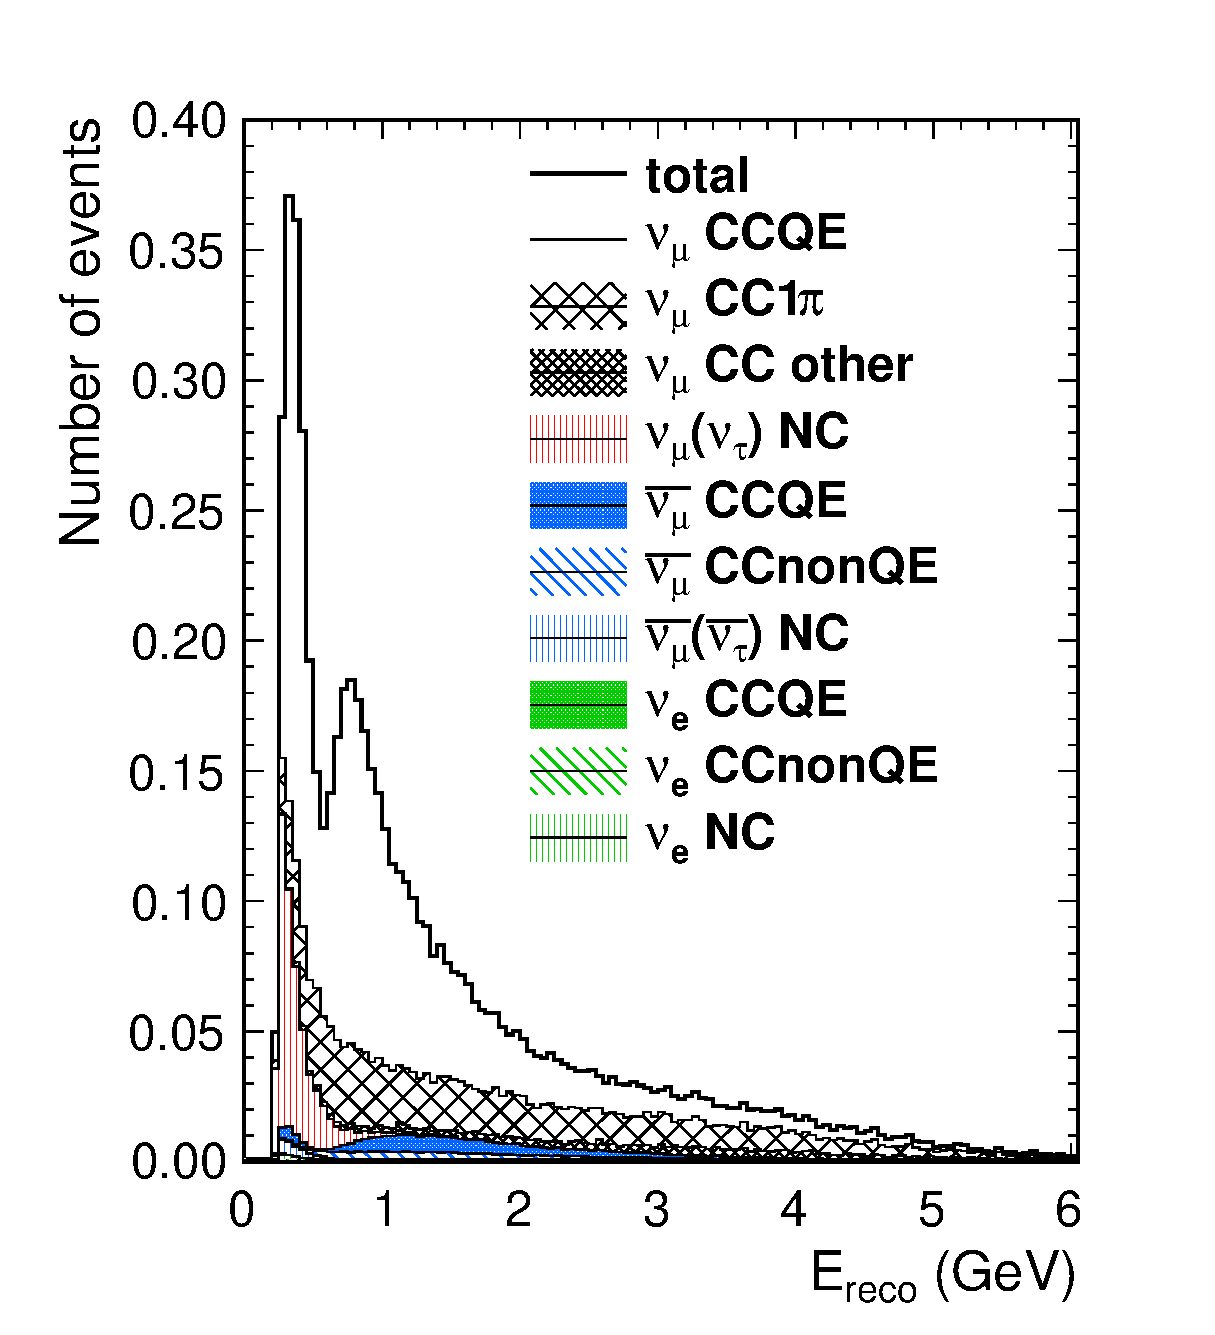
\includegraphics[width=19pc,height=19pc]{./images/predicted_spectrum/nominal/genie_contrib_2p4Em3_1p0.eps}
\caption{
  Predicted oscillated ($sin^{2}2\theta_{23}$ = 1.0 and $\Delta m^{2}_{23}$ = 2.4$\times10^{-3}$ $eV^{2}/c^{4}$) 
  reconstructed-energy spectrum of 1-ring $\mu$-like events (after extrapolation)
  and contributions from various true neutrino reaction modes (GENIE).
}
\label{fig:genie_mode_contrib_2p4Em3_1p0}
\end{minipage}
\hspace{0.04\linewidth}
\begin{minipage}[t]{0.48\linewidth}
\centering
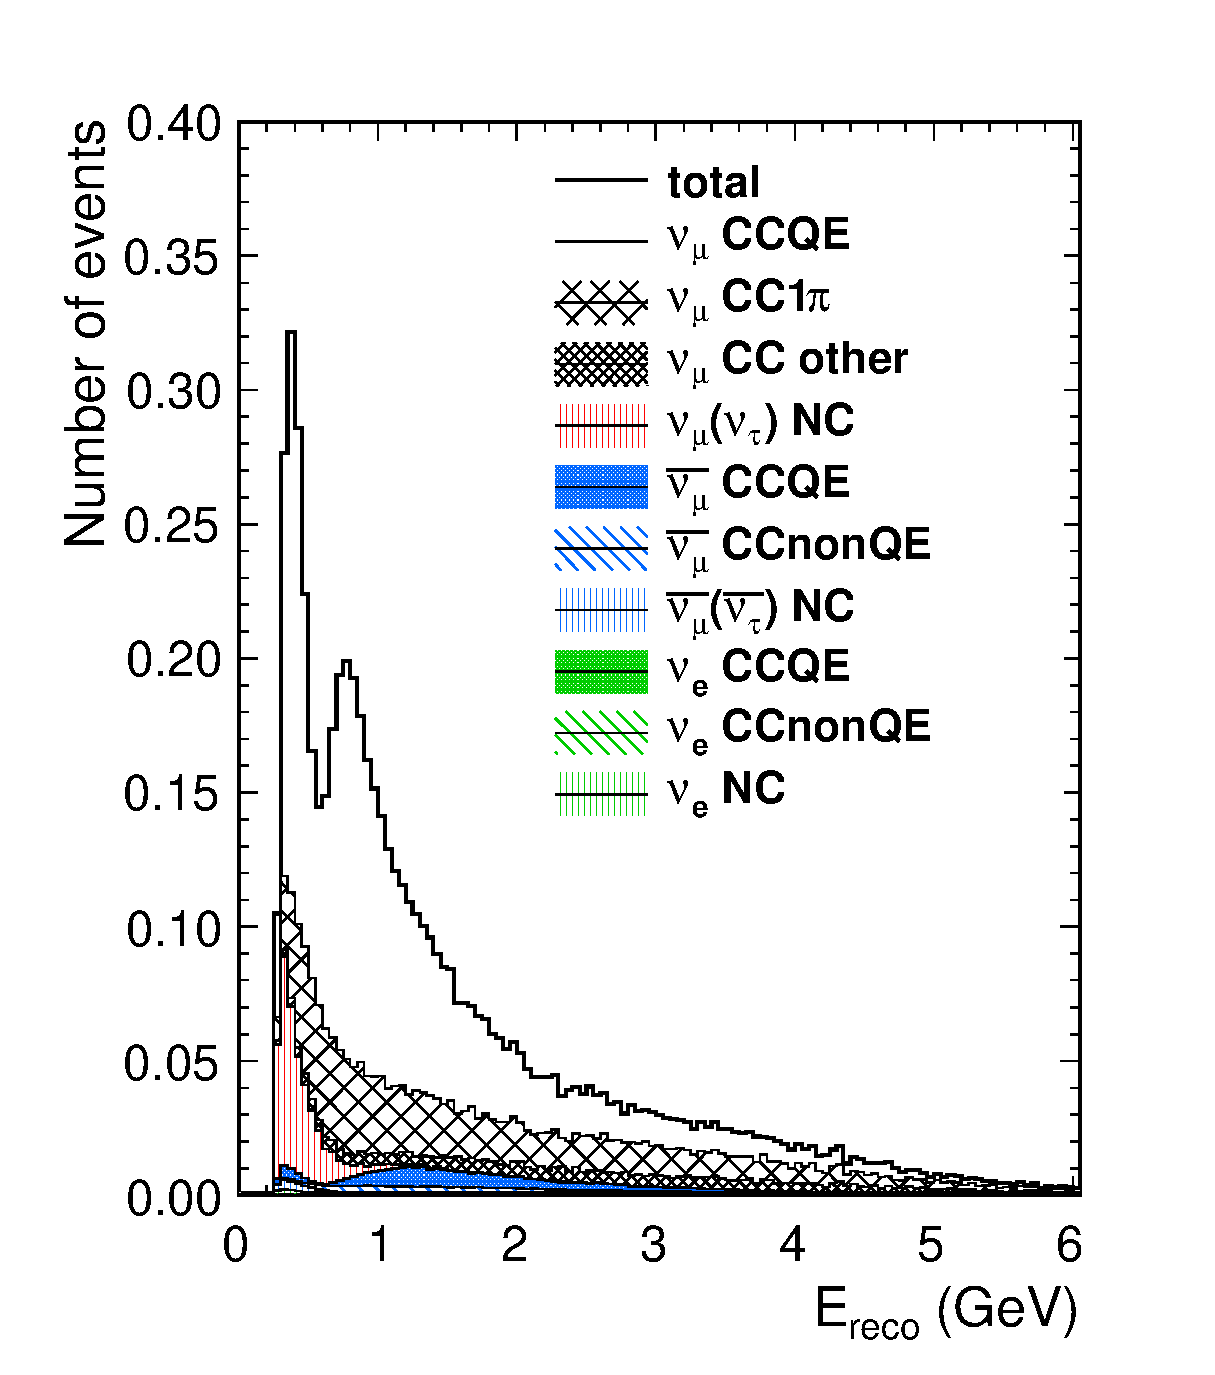
\includegraphics[width=19pc,height=19pc]{images/predicted_spectrum/nominal/neut_contrib_2p4Em3_1p0.eps}
\caption{
  Predicted oscillated ($sin^{2}2\theta_{23}$ = 1.0 and $\Delta m^{2}_{23}$ = 2.4$\times10^{-3}$ $eV^{2}/c^{4}$) 
  reconstructed-energy spectrum of 1-ring $\mu$-like events (after extrapolation)
  and contributions from various true neutrino reaction modes (NEUT).
}
\label{fig:neut_mode_contrib_2p4Em3_1p0}
\end{minipage}
\end{figure}



\begin{table}
\centering
\begin{tabular}{| c || c | c || c | c | }
\hline
   & \multicolumn{2}{c||} { (a) } 
   & \multicolumn{2}{c| } { (b) }\\
                                         & GENIE              & NEUT               & GENIE               & NEUT  \\
\hline
\hline
Total                                    &  22.4193            &  22.8136            &  6.2043             &    6.3395             \\
$\nu_{\mu}$ CCQE                         &  18.0269 (80.408\%) &  18.0707 (79.210\%) &  3.5785 (57.678\%)  &    3.5944 (56.699\%)   \\
$\nu_{\mu}$ CC1$\pi$                     &   2.8527 (12.724\%) &   3.0883 (13.537\%) &  1.4488 (23.352\%)  &    1.5163 (23.918\%)   \\
$\nu_{\mu}$ CCother                      &   0.2995  (1.336\%) &   0.5219 (2.288\%)  &  0.2514  (4.052\%)  &    0.4056 (6.398\%)   \\
$\nu_{\mu}$($\nu_{\tau}$) NC             &   0.4720  (2.106\%) &   0.3767 (1.651\%)  &  0.4720  (7.608\%)  &    0.3767 (5.942\%)   \\
$\bar{\nu_{\mu}}$ CCQE                   &   0.4854  (2.165\%) &   0.5027 (2.203\%)  &  0.2375  (3.828\%)  &    0.2526 (3.985\%)   \\
$\bar{\nu_{\mu}}$ CCnonQE                &   0.2383  (1.063\%) &   0.2160 (0.947\%)  &  0.1716  (2.765\%)  &    0.1564 (2.468\%)   \\
$\bar{\nu_{\mu}}$($\bar{\nu_{\tau}}$) NC &   0.0273  (0.122\%) &   0.0219 (0.096\%)  &  0.0273  (0.440\%)  &    0.0219 (0.345\%)   \\
$\nu_{e}$ CCQE                           &   0.0016  (0.007\%) &   0.0017 (0.008\%)  &  0.0016  (0.026\%)  &    0.0017 (0.027\%)   \\
$\nu_{e}$ CCnonQE                        &   0.0012  (0.005\%) &   0.0015 (0.006\%)  &  0.0012  (0.020\%)  &    0.0015 (0.023\%)   \\
$\nu_{e}$ NC                             &   0.0144  (0.064\%) &   0.0124 (0.054\%)  &  0.0144  (0.232\%)  &    0.0124 (0.195\%)   \\
\hline
\end{tabular}
\caption{
  Expected numbers of SuperK 1-ring $\mu$-like events from GENIE and NEUT (after extrapolation) for 
  (a) no oscillation and 
  (b) oscillations with $sin^{2}2\theta_{23}$ = 1.0 and $\Delta m^{2}_{23}$ = 2.4$\times10^{-3}$ $eV^{2}/c^{4}$.
}
\label{tab:genie_neut_mode_contrib}
\end{table}



\begin{figure}[ht]
\begin{minipage}[t]{0.47\linewidth}
\centering
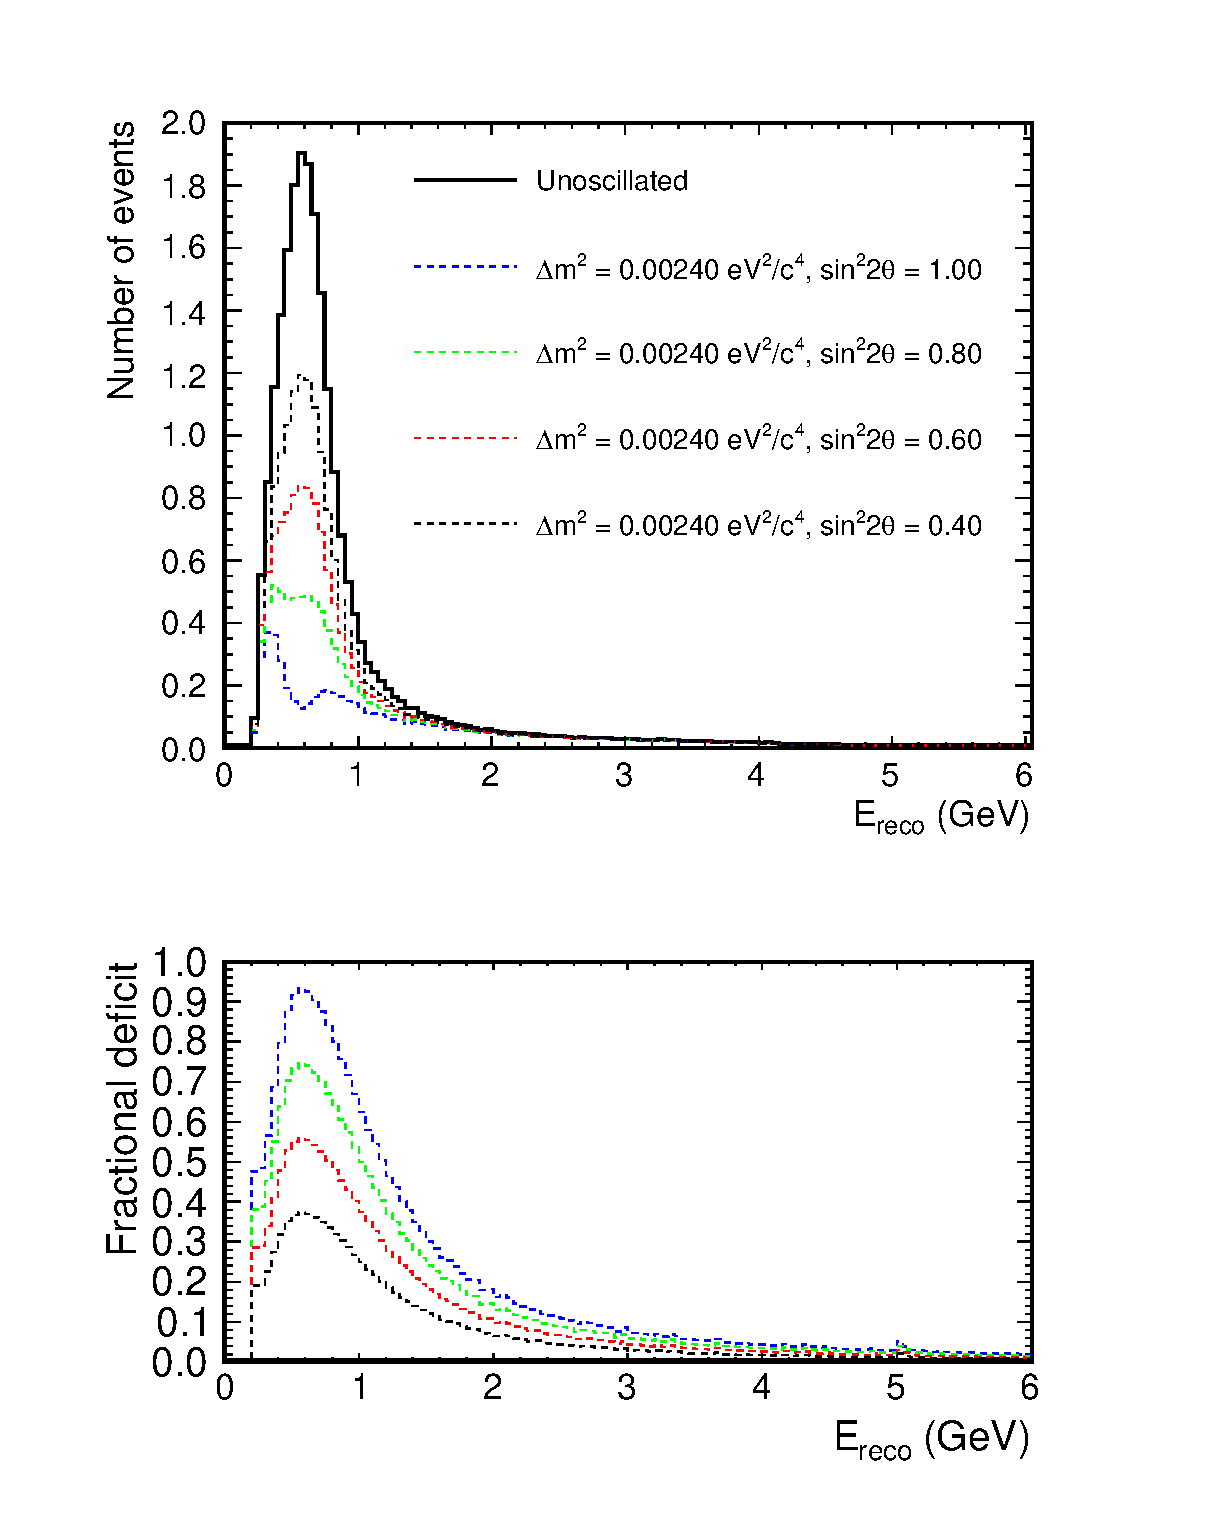
\includegraphics[width=19pc,height=22pc]{./images/predicted_spectrum/nominal/genie_sk_spectrum_2p4Em3_twk_sinsq2theta.eps}
\caption{
  Predicted reconstructed-energy spectrum of 1-ring $\mu$-like events (after extrapolation)
  for $\Delta m^{2}_{23}$ = 2.4$\times10^{-3}$ $eV^{2}/c^{4}$ and
  $sin^{2}2\theta_{23}$ = 1.0, 0.8, 0.6, 0.4. 
  The non-oscillated spectrum is also shown (GENIE).
}
\label{fig:genie_sk_spectrum_twk_sinsq2theta}
\end{minipage}
\hspace{0.06\linewidth}
\begin{minipage}[t]{0.47\linewidth}
\centering
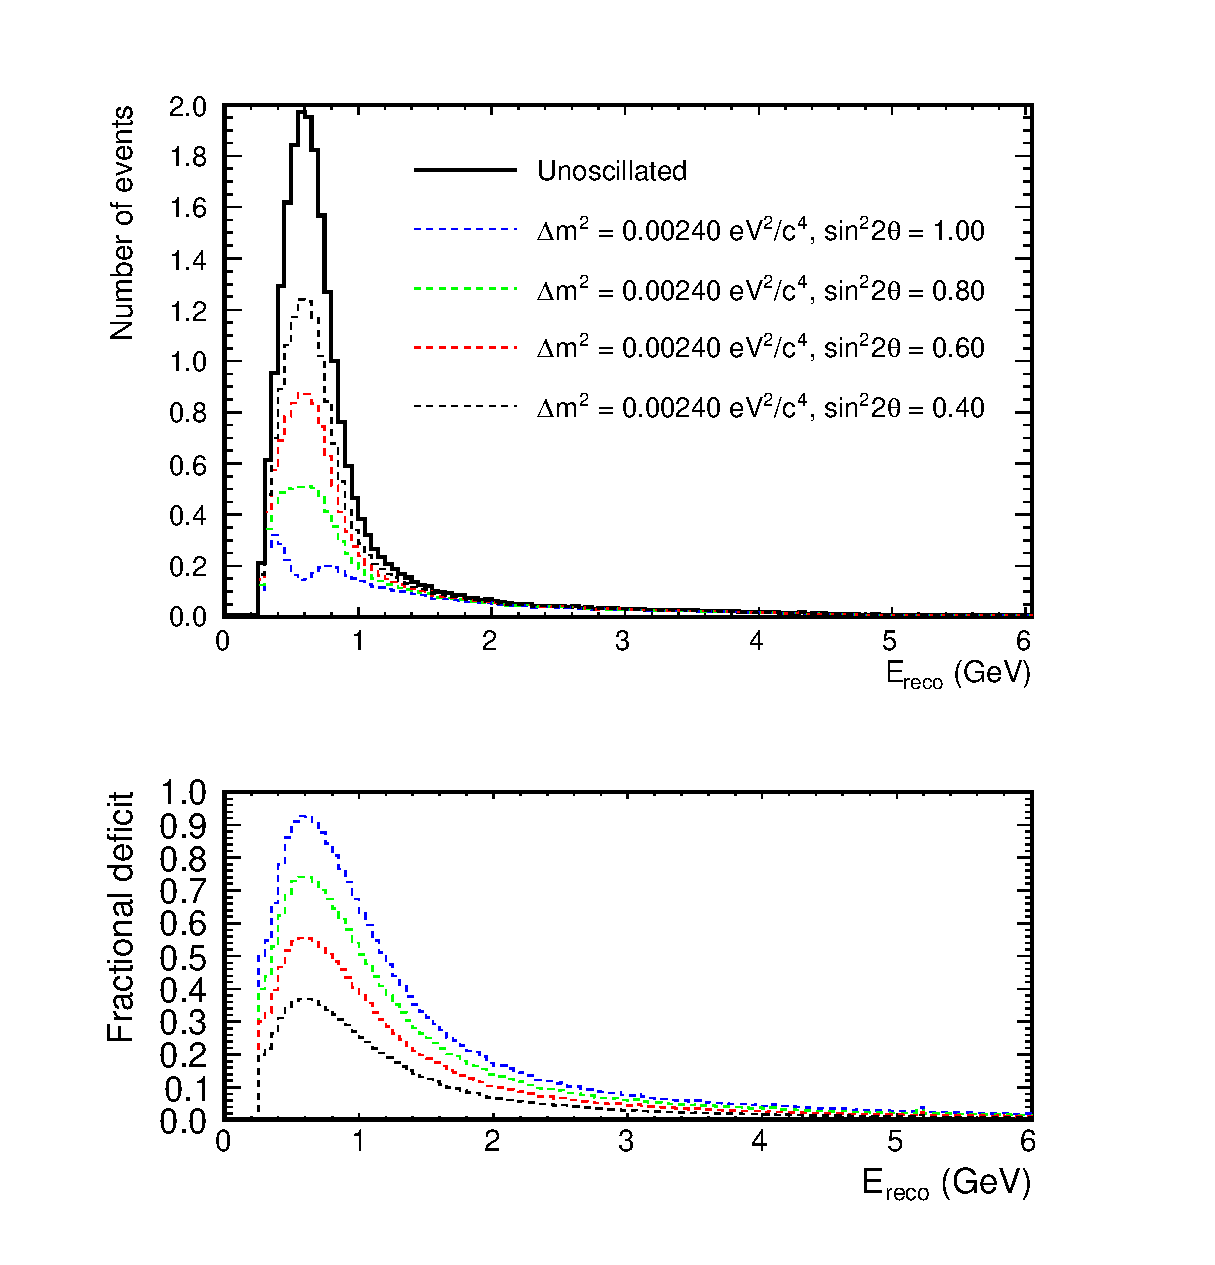
\includegraphics[width=19pc,height=22pc]{images/predicted_spectrum/nominal/neut_sk_spectrum_2p4Em3_twk_sinsq2theta.eps}
\caption{
  Predicted reconstructed-energy spectrum of 1-ring $\mu$-like events (after extrapolation)
  for $\Delta m^{2}_{23}$ = 2.4$\times10^{-3}$ $eV^{2}/c^{4}$ and
  $sin^{2}2\theta_{23}$ = 1.0, 0.8, 0.6, 0.4. 
  The non-oscillated spectrum is also shown (NEUT).
}
\label{fig:neut_sk_spectrum_twk_sinsq2theta}
\end{minipage}
\end{figure}


\begin{table}
\centering
\begin{tabular}{| c | c | c | c | c | c | c | c | c | c | c | }
\hline
$E_{reco}$
   & \multicolumn{2}{c|} { (a) } 
   & \multicolumn{2}{c|} { (b) }
   & \multicolumn{2}{c|} { (c) }
   & \multicolumn{2}{c|} { (d) }
   & \multicolumn{2}{c|} { (e) }\\
           (GeV) & GENIE  & NEUT     & GENIE  & NEUT     & GENIE  & NEUT    & GENIE  & NEUT    & GENIE  & NEUT  \\
\hline
\hline
$<$  0.50        &  7.442 &  6.526   &  1.691 &  1.379   &  2.841 &  2.408  &  3.991 &  3.438  &  5.142 &  4.467 \\
$<$  0.75        & 15.528 & 15.114   &  2.490 &  2.239   &  5.098 &  4.814  &  7.705 &  7.389  & 10.313 &  9.964 \\
$<$  1.00        & 18.392 & 18.315   &  3.252 &  3.065   &  6.280 &  6.115  &  9.308 &  9.165  & 12.336 & 12.215 \\
$<$  1.50        & 20.101 & 20.245   &  4.180 &  4.100   &  7.364 &  7.329  & 10.548 & 10.558  & 13.732 & 13.787 \\
$<$  2.00        & 20.839 & 21.063   &  4.751 &  4.729   &  7.969 &  7.996  & 11.186 & 11.263  & 14.404 & 14.592 \\
$<$  4.00        & 22.068 & 22.417   &  5.864 &  5.956   &  9.105 &  9.248  & 12.346 & 12.540  & 15.586 & 15.833 \\
$<$ 10.00        & 22.419 & 22.814   &  6.204 &  6.340   &  9.447 &  9.634  & 12.690 & 12.929  & 15.933 & 16.224 \\
\hline
\end{tabular}
\caption{
  Expected numbers of SuperK 1-ring $\mu$-like events from GENIE and NEUT (after extrapolation) for
  various reconstructed energy slices and oscillation hypotheses.
  The non-oscillated expectations are shown in (a), while (b)-(e) show the oscillated expectation 
  for $\Delta m^{2}_{23}$ = 2.4$\times10^{-3}$ $eV^{2}/c^{4}$ 
  and various neutrino mixing angles:
  (b) $sin^{2}2\theta_{23}$ = 1.0,
  (c) $sin^{2}2\theta_{23}$ = 0.8, 
  (d) $sin^{2}2\theta_{23}$ = 0.6 and 
  (e) $sin^{2}2\theta_{23}$ = 0.4.
}
\label{tab:genie_neut_nsk_twk_sinsq2theta}
\end{table}



\begin{figure}[ht]
\begin{minipage}[t]{0.47\linewidth}
\centering
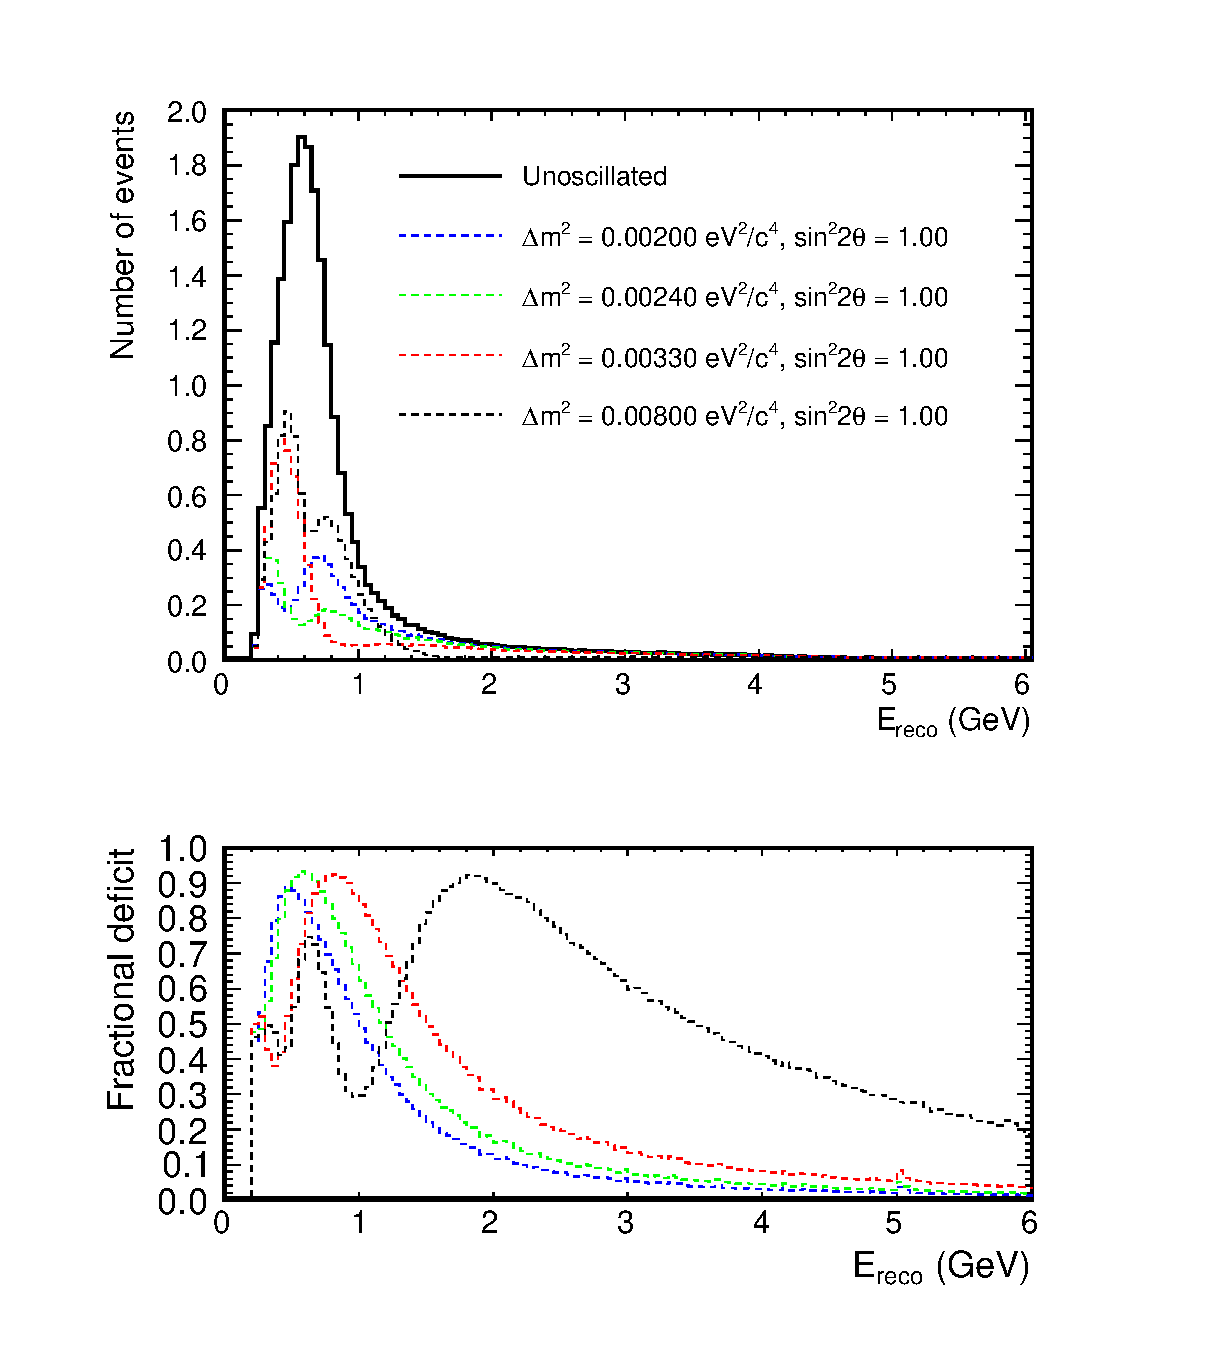
\includegraphics[width=19pc,height=22pc]{./images/predicted_spectrum/nominal/genie_sk_spectrum_1p0_twk_dmsq.eps}
\caption{
  Predicted reconstructed-energy spectrum of 1-ring $\mu$-like events (after extrapolation)
  for $sin^{2}2\theta_{23}$ = 1.0 and  
  $\Delta m^{2}_{23}$ =
    2.0$\times10^{-3}$ $eV^{2}/c^{4}$,
    2.4$\times10^{-3}$ $eV^{2}/c^{4}$,
    3.3$\times10^{-3}$ $eV^{2}/c^{4}$ and
    8.0$\times10^{-3}$ $eV^{2}/c^{4}$.
  The non-oscillated spectrum is also shown (GENIE).
}
\label{fig:genie_sk_spectrum_twk_dmsq}
\end{minipage}
\hspace{0.06\linewidth}
\begin{minipage}[t]{0.47\linewidth}
\centering
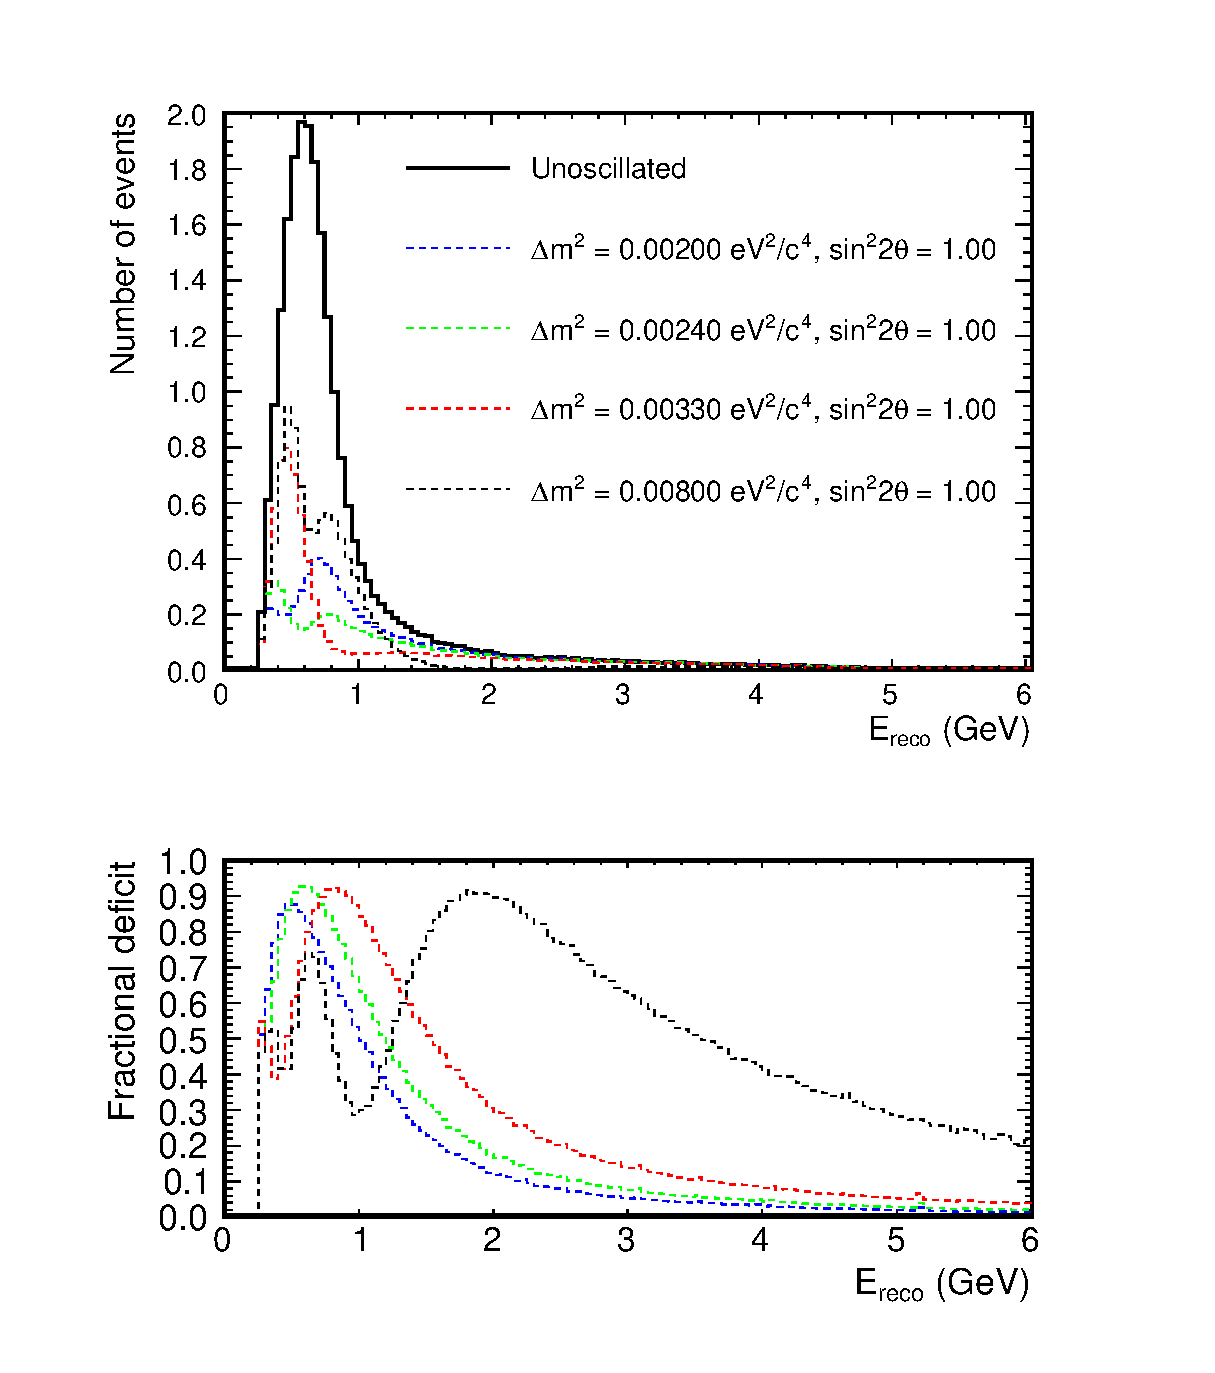
\includegraphics[width=19pc,height=22pc]{images/predicted_spectrum/nominal/neut_sk_spectrum_1p0_twk_dmsq.eps}
\caption{
  Predicted reconstructed-energy spectrum of 1-ring $\mu$-like events (after extrapolation)
  for $sin^{2}2\theta_{23}$ = 1.0 and  
  $\Delta m^{2}_{23}$=
    2.0$\times10^{-3}$ $eV^{2}/c^{4}$,
    2.4$\times10^{-3}$ $eV^{2}/c^{4}$,
    3.3$\times10^{-3}$ $eV^{2}/c^{4}$ and
    8.0$\times10^{-3}$ $eV^{2}/c^{4}$.
  The non-oscillated spectrum is also shown (NEUT).
}
\label{fig:neut_sk_spectrum_twk_dmsq}
\end{minipage}
\end{figure}



\begin{table}
\centering
\begin{tabular}{| c | c | c | c | c | c | c | c | c | c | c | }
\hline
$E_{reco}$
   & \multicolumn{2}{c|} { (a) } 
   & \multicolumn{2}{c|} { (b) }
   & \multicolumn{2}{c|} { (c) }
   & \multicolumn{2}{c|} { (d) }
   & \multicolumn{2}{c|} { (e) }\\
           (GeV) & GENIE  & NEUT     & GENIE  & NEUT     & GENIE  & NEUT    & GENIE  & NEUT    & GENIE  & NEUT  \\
\hline
\hline
$<$  0.50        &  7.442 &  6.526   &  1.416 &  1.170   &  1.691 &  1.379  &  3.752 &  3.252  &  3.919 &  3.245 \\
$<$  0.75        & 15.528 & 15.114   &  3.128 &  2.977   &  2.490 &  2.239  &  5.070 &  4.718  &  6.501 &  6.189 \\
$<$  1.00        & 18.392 & 18.315   &  4.303 &  4.264   &  3.252 &  3.065  &  5.357 &  5.038  &  8.336 &  8.203 \\
$<$  1.50        & 20.101 & 20.245   &  5.421 &  5.516   &  4.180 &  4.100  &  5.909 &  5.647  &  9.136 &  9.139 \\
$<$  2.00        & 20.839 & 21.063   &  6.039 &  6.198   &  4.751 &  4.729  &  6.364 &  6.145  &  9.213 &  9.231 \\
$<$  4.00        & 22.068 & 22.417   &  7.186 &  7.462   &  5.864 &  5.956  &  7.385 &  7.269  &  9.623 &  9.672 \\
$<$ 10.00        & 22.419 & 22.814   &  7.529 &  7.850   &  6.204 &  6.340  &  7.716 &  7.641  &  9.868 &  9.947 \\
\hline
\end{tabular}
\caption{
  Expected numbers of SuperK 1-ring $\mu$-like events from GENIE and NEUT (after extrapolation) for
  various reconstructed energy slices and oscillation hypotheses.
  The non-oscillated expectations are shown in (a), while (b)-(e) show the oscillated expectation 
  for $sin^{2}2\theta_{23}$ = 1.0
  and squared neutrino mass differences:
  (b) $\Delta m^{2}_{23}$ = 2.0$\times10^{-3}$ $eV^{2}/c^{4}$,
  (c) $\Delta m^{2}_{23}$ = 2.4$\times10^{-3}$ $eV^{2}/c^{4}$,
  (d) $\Delta m^{2}_{23}$ = 3.3$\times10^{-3}$ $eV^{2}/c^{4}$ and
  (e) $\Delta m^{2}_{23}$ = 8.0$\times10^{-3}$ $eV^{2}/c^{4}$
}
\label{tab:genie_neut_nsk_twk_dmsq}
\end{table}


\begin{figure}[ht]
\begin{minipage}[t]{0.47\linewidth}
\centering
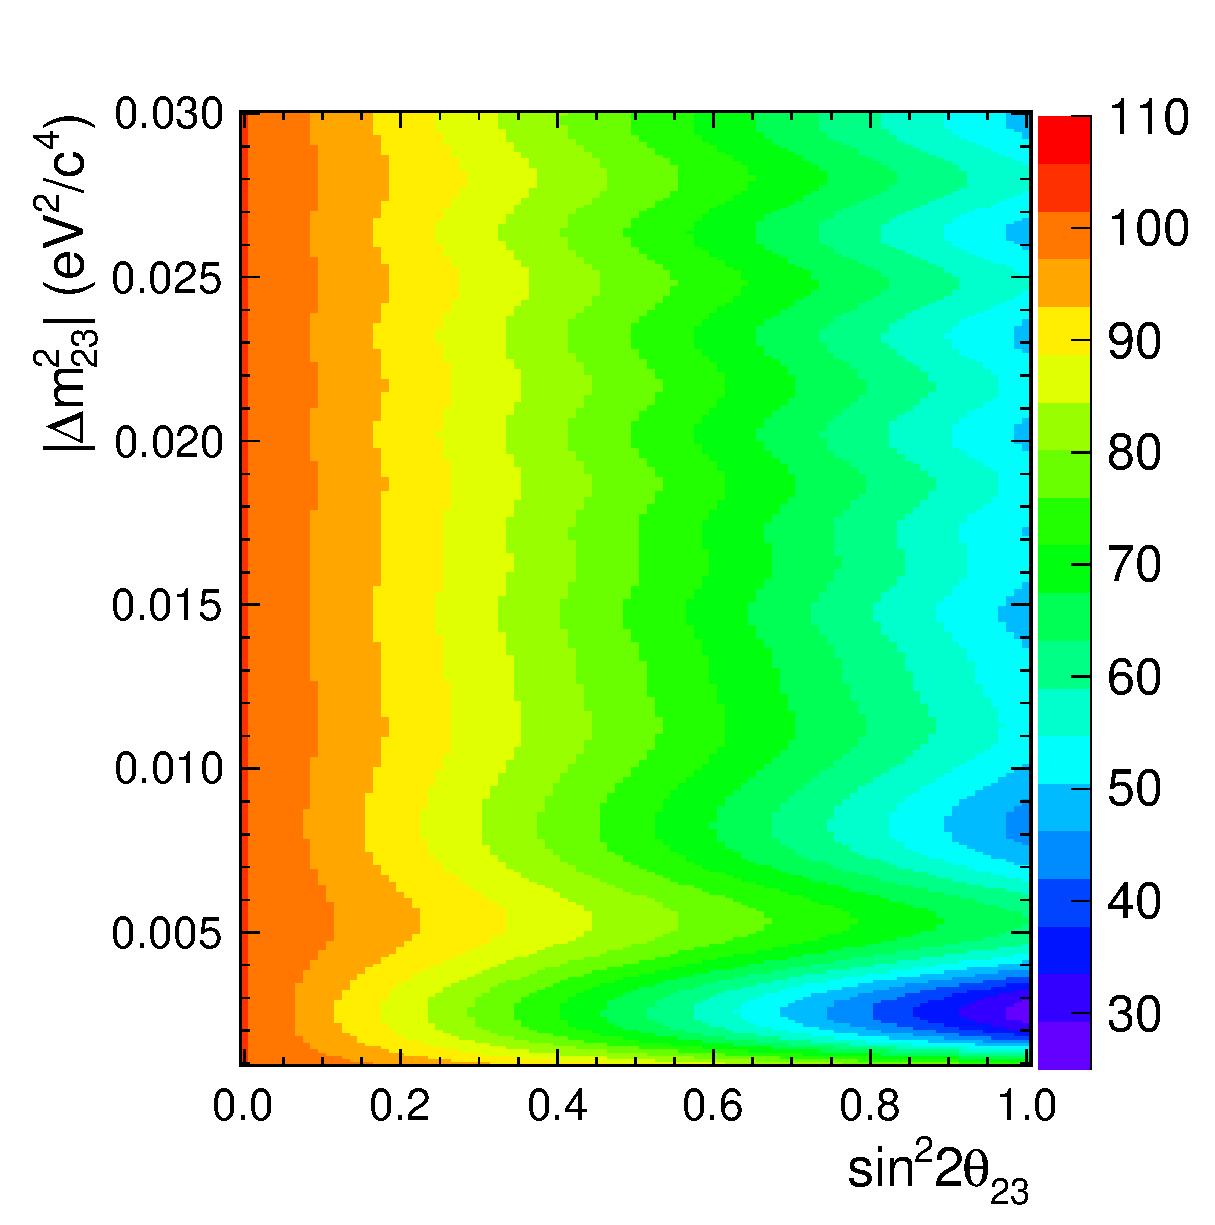
\includegraphics[width=18pc,height=16pc]{./images/predicted_spectrum/nominal/genie_nsk_osc.eps}
\caption{
  Expected number of 1-ring $\mu$-like events (after extrapolation) in the 0-10 GeV reconstructed 
  energy range (GENIE).
}
\label{fig:genie_nsk_osc_param_grid}
\end{minipage}
\hspace{0.06\linewidth}
\begin{minipage}[t]{0.47\linewidth}
\centering
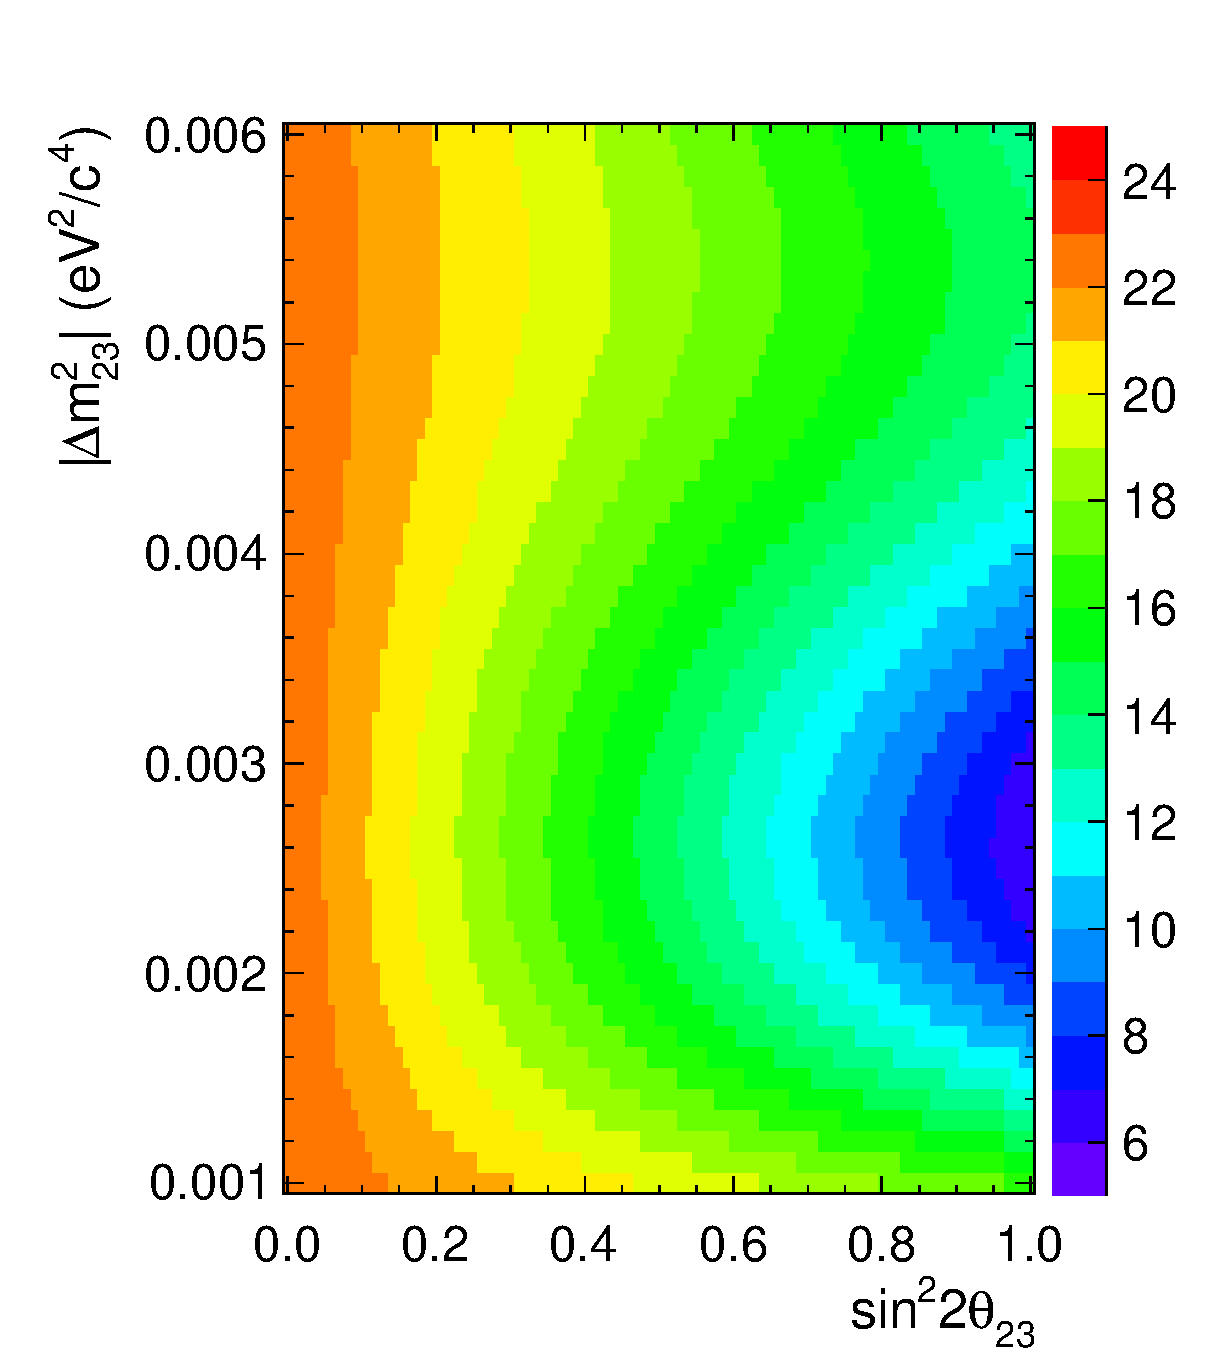
\includegraphics[width=17pc,height=16pc]{images/predicted_spectrum/nominal/neut_nsk_osc.eps}
\caption{
  Expected number of 1-ring $\mu$-like events (after extrapolation) in the 0-10 GeV reconstructed 
  energy range (NEUT).
}
\label{fig:neut_nsk_osc_param_grid}
\end{minipage}
\end{figure}


\begin{figure*}[htb]
\center
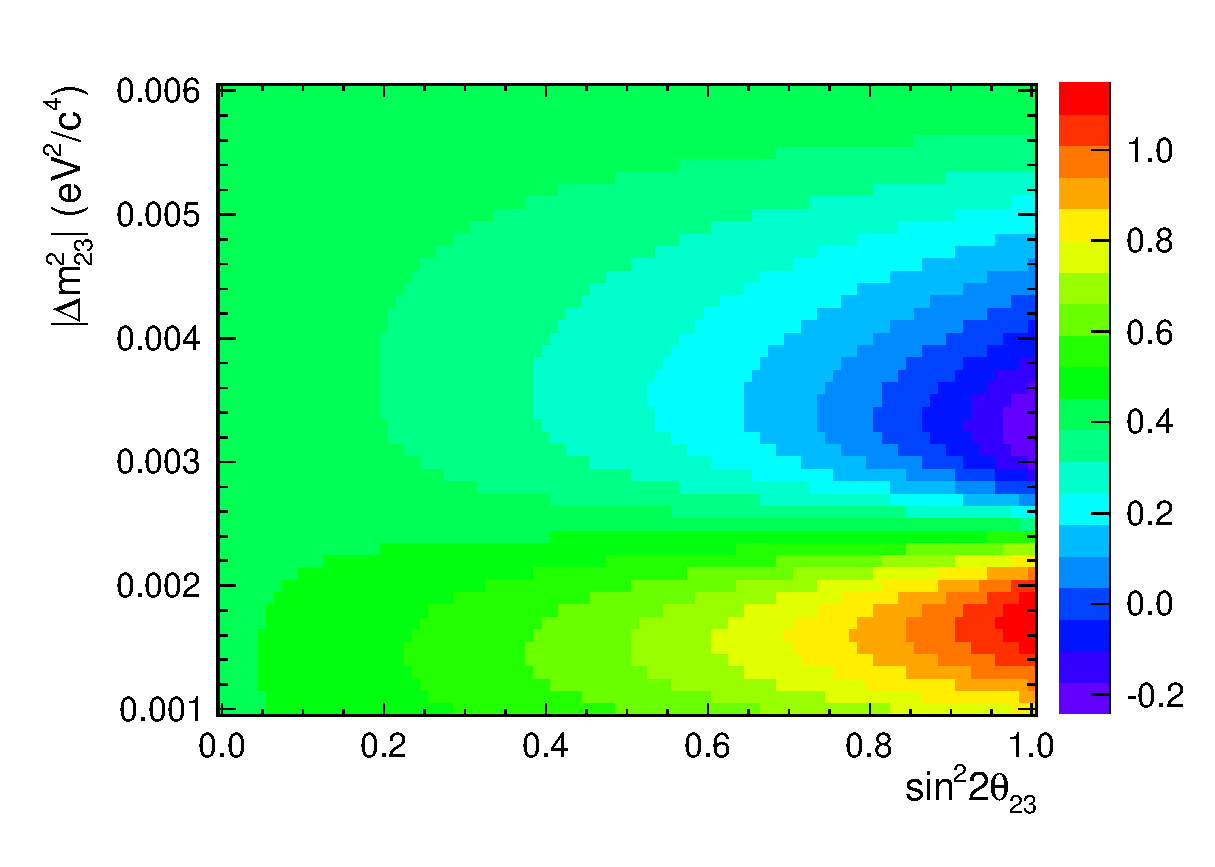
\includegraphics[width=38pc]{./images/predicted_spectrum/nominal/genie_neut_nsk_diff_osc.eps}
\caption{
  Percentage difference $100\cdot(N^{NEUT}_{SK}-N^{GENIE}_{SK})/(N^{NEUT}_{SK}+N^{GENIE}_{SK})/2$ 
  between the GENIE and NEUT
  expected numbers of 1-ring $\mu$-like events (after extrapolation) 
  in the 0-10 GeV reconstructed energy range. 
  The percentage difference in the -0.2\% to +1.2\% range
  (Compare with Fig. \ref{fig:nsk_uncertainty_osc_param_grid_xsec_err_only}).
}
\label{fig:genie_neut_nsk_difference_osc_param_grid}
\end{figure*}
